% This text is proprietary.
% It's a part of presentation made by myself.
% It may not used commercial.
% The noncommercial use such as private and study is free
% Dec 2007
% Author: Sascha Frank 
% University Freiburg 
% www.informatik.uni-freiburg.de/~frank/
%
% 
\documentclass{beamer}
\setbeamertemplate{navigation symbols}{}

%\setbeamercolor{frametitle}{fg=black,bg=white}
%\setbeamercolor{title}{fg=black,bg=yellow!85!orange}
\usetheme{AnnArbor}
\usecolortheme{beaver}
\usefonttheme{structurebold}


\usepackage{algorithm}
\usepackage{algorithmic}
\usepackage{multicol}
\usepackage{bbold}
\usepackage{graphicx}

\beamersetuncovermixins{\opaqueness<1>{25}}{\opaqueness<2->{15}}
\begin{document}
\title{Community Detection}
\subtitle{In Large Networks}
\author{June Andrews}
\institute{Cornell University}
\date{\today} 

\begin{frame}
\titlepage
\end{frame}


\begin{frame}\frametitle{Thanks!}
It goes without saying, these people have been inspiring forces of nature to work with:
\begin{itemize}
\item Mr. Len Kulbacki
\item Coach Wilson
\item Dr. James Sethian
\item Patricia Kovatch
\item Dr. Alex Vladimirsky
\item Dr. John Hopcroft
\item Dr. Steve Strogatz (thanks to Prof Rand for acting proxy :)
\item Dr. Jon Kleinberg
\end{itemize}

\begin{figure}

\includegraphics[width=.7in]{Figures/nsflogo} 
\caption{Thanks to the NSF Graduate Fellowship Program!}
\end{figure}

\end{frame}

\begin{frame}\frametitle{Table of contents}\tableofcontents
\end{frame} 


\section{Motivation}



\begin{frame}\frametitle{Applications In General}

\begin{table}[ht]
\centering
\begin{tabular}{p{.9in} p{.1in} p{1.3in} p{.1in} p{2in}}
Build Network &  & Find Communities &  & Analyze \\
& $\rightarrow$ & & $\rightarrow$ & \\
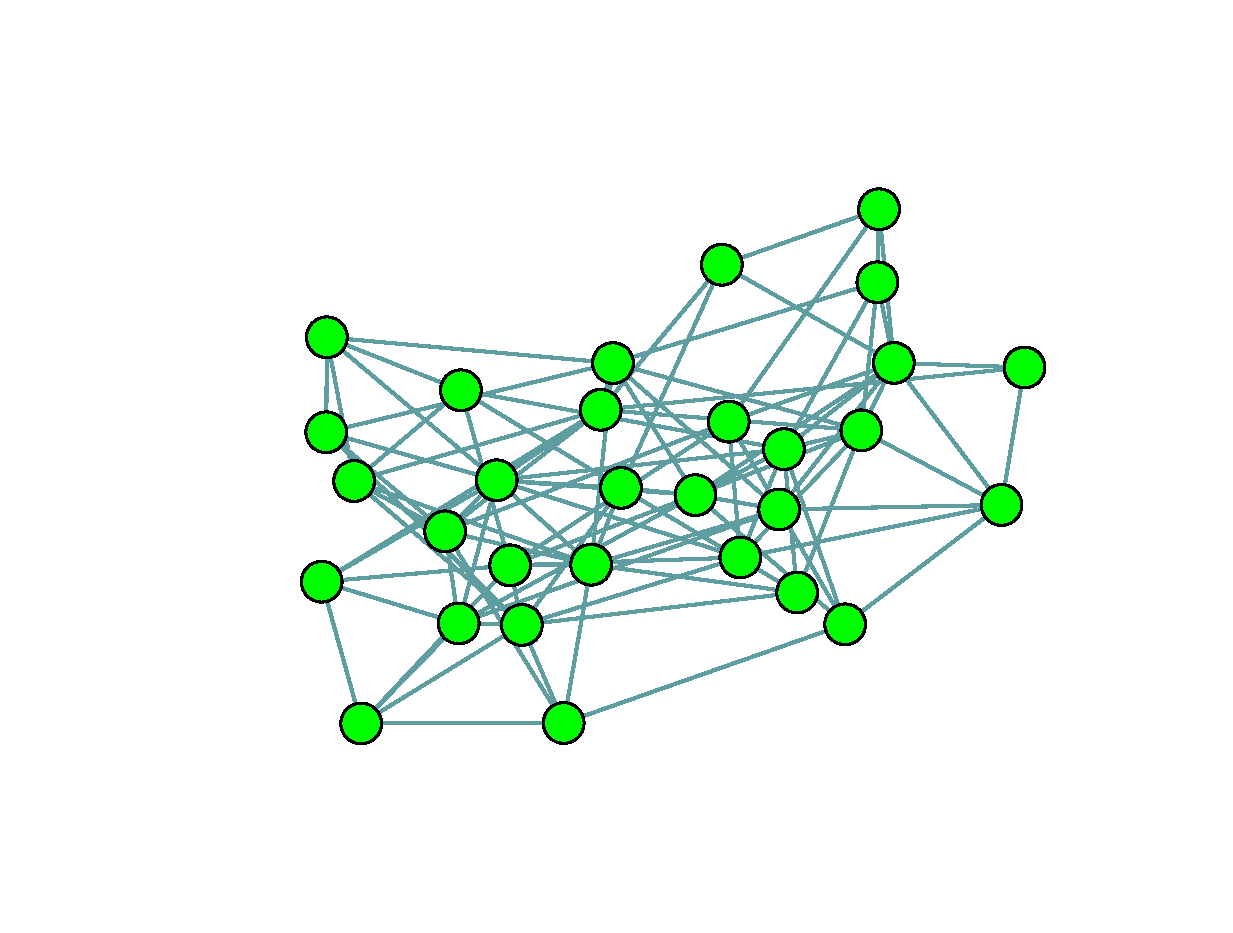
\includegraphics[width=1.3in]{Figures/random_graph} &  & 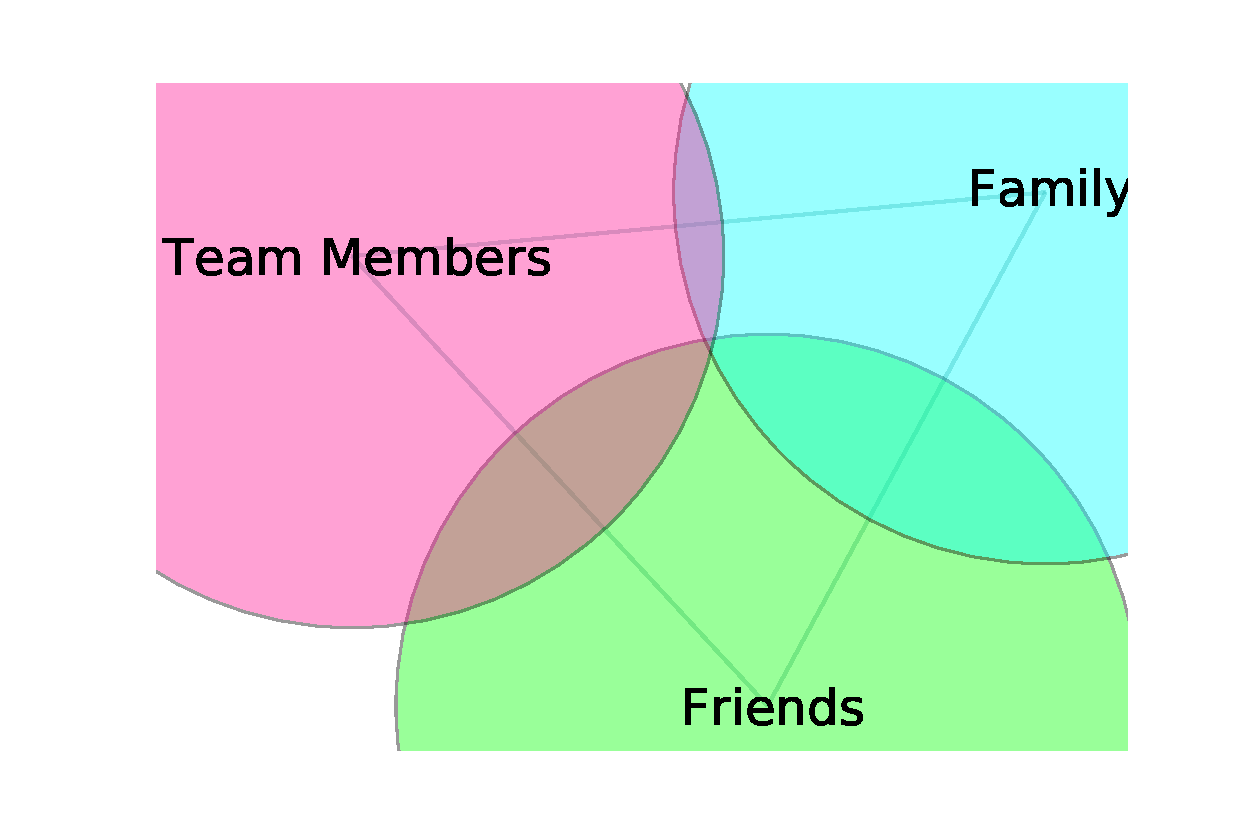
\includegraphics[width=1.3in]{Figures/abstract_community} &  & Who are the leaders? \newline How do groups interact? \newline 
\end{tabular}
\end{table}


\begin{block}{}
\begin{center}
How do you detect communities?
\end{center}
\end{block}

\end{frame}


\begin{frame}\frametitle{Dolphins}
Dolphins form pods.
\begin{figure}
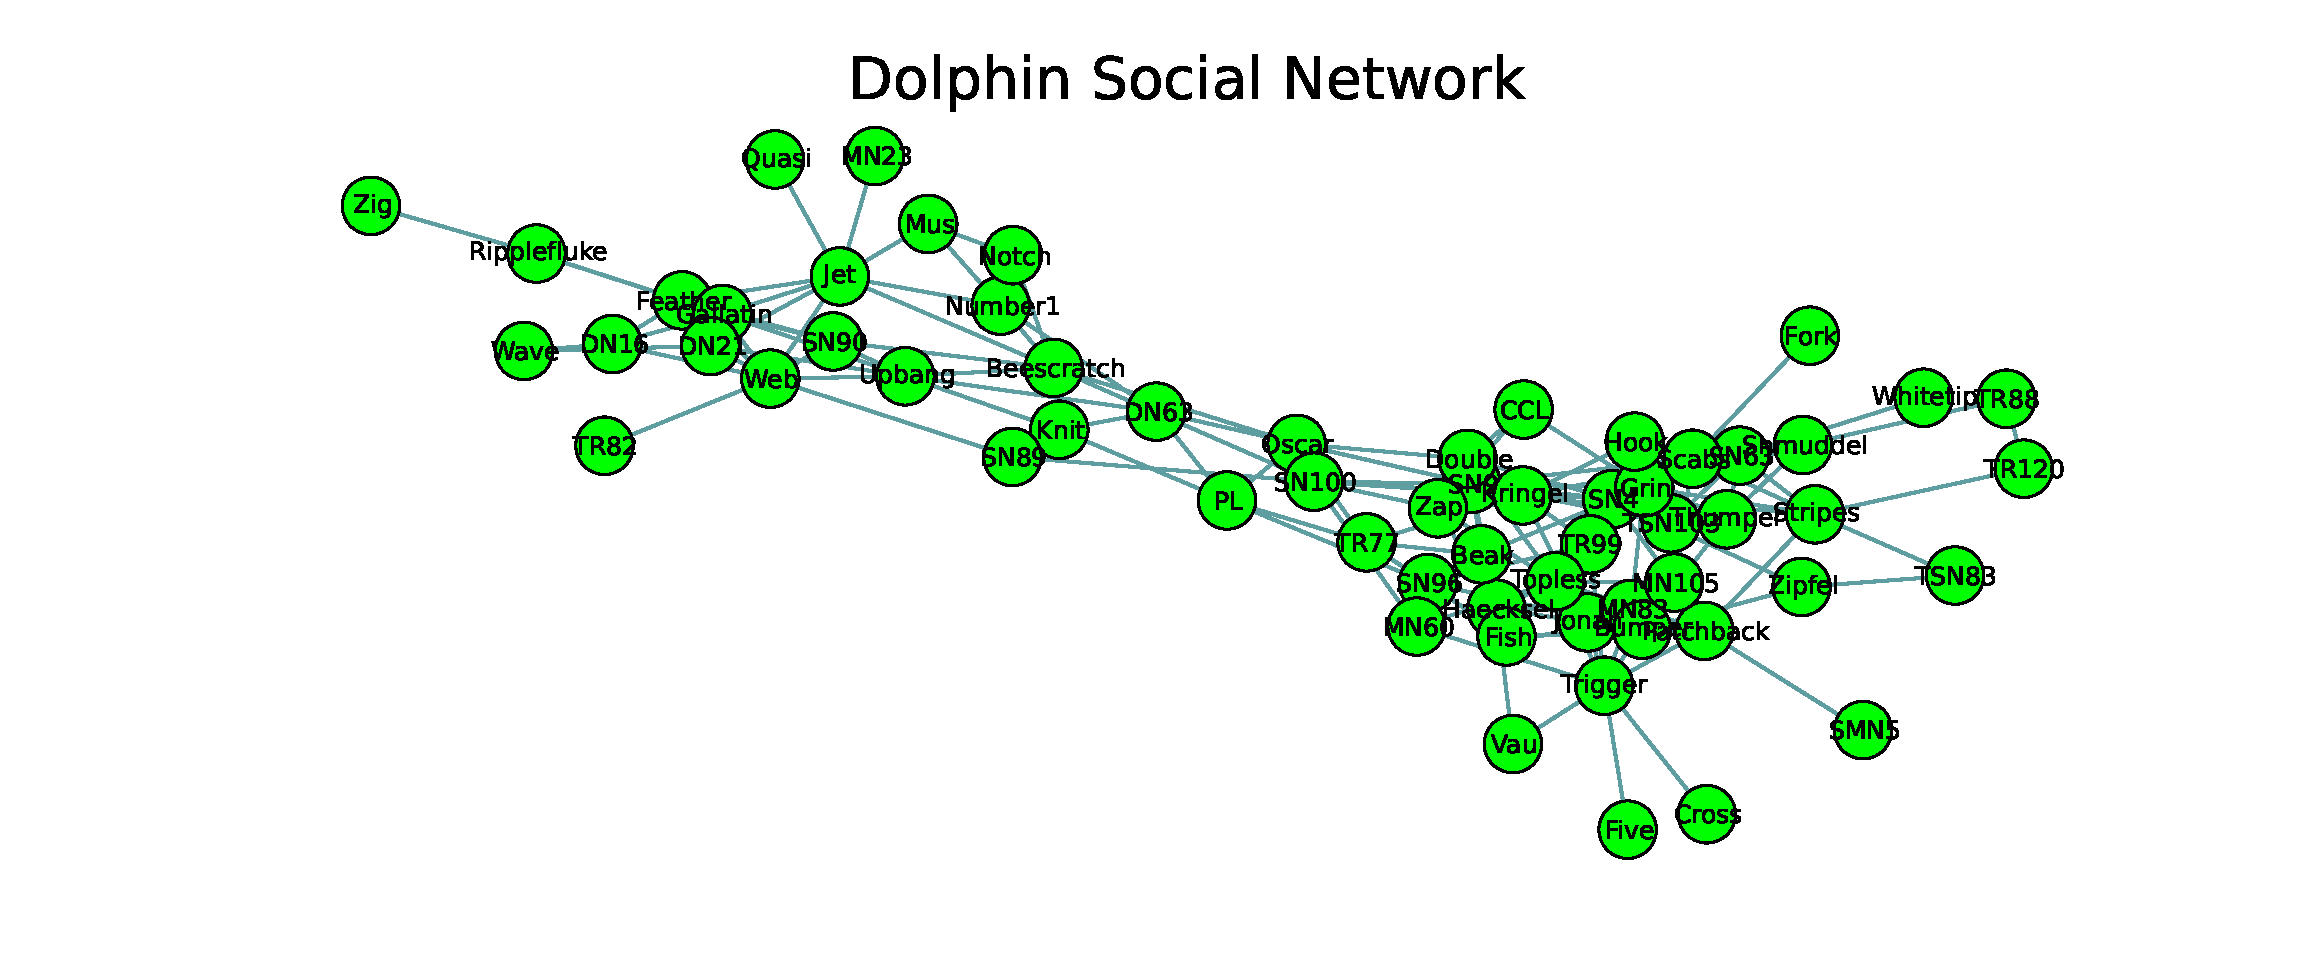
\includegraphics[width=5in]{Figures/dolphin_social_network}
\caption{Nodes are dolphins.  Edges are dolphins seen together.}
\end{figure}
\end{frame}

\begin{frame}\frametitle{Dolphins}
If we know what the pods are:
\begin{itemize}
\item Who are the dolphins that interact between pods?
\item How often do pods interact?
\item Do the pods have a dominant leader?
\end{itemize}
\begin{figure}
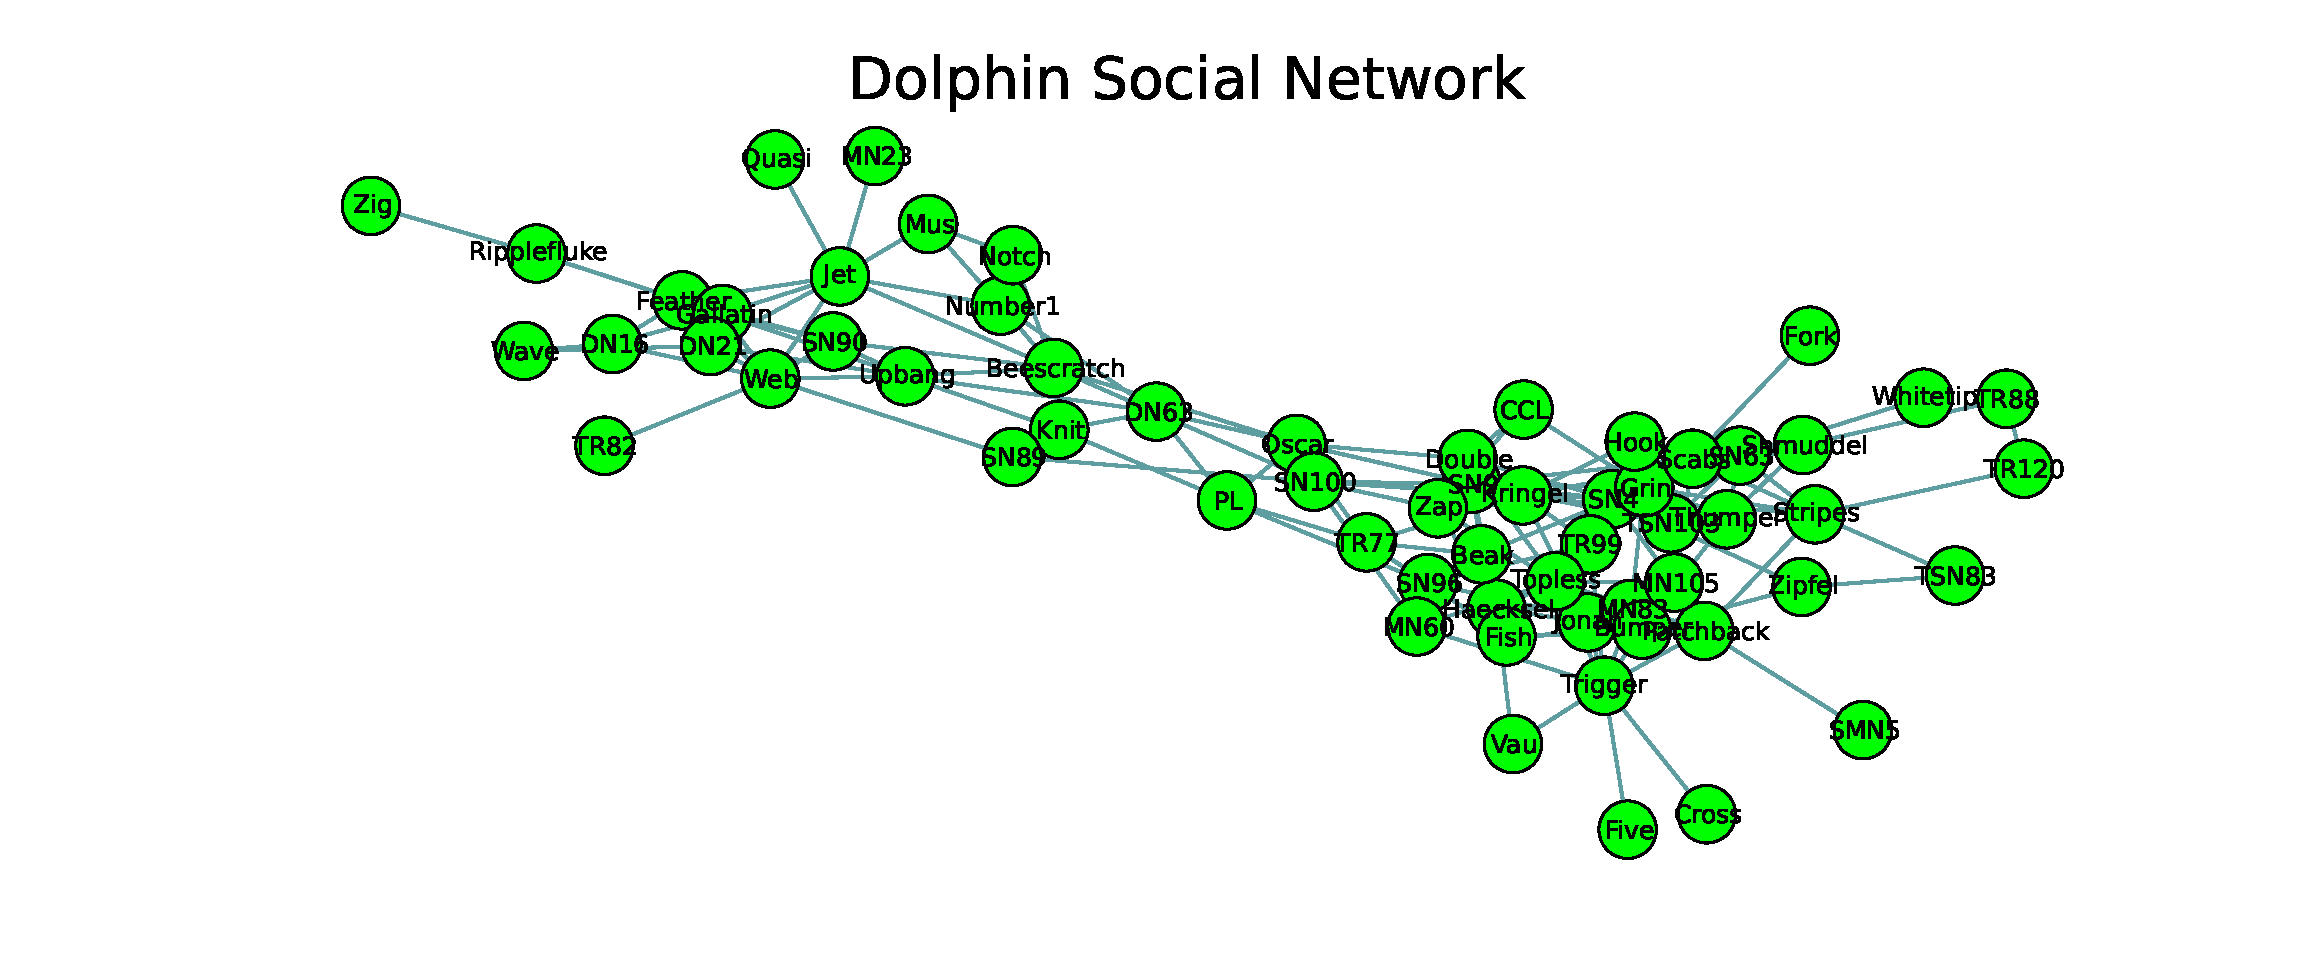
\includegraphics[width=3in]{Figures/dolphin_social_network}
\end{figure}
\end{frame}


\begin{frame}\frametitle{Karate Club}
People are members of a group.
\begin{figure}
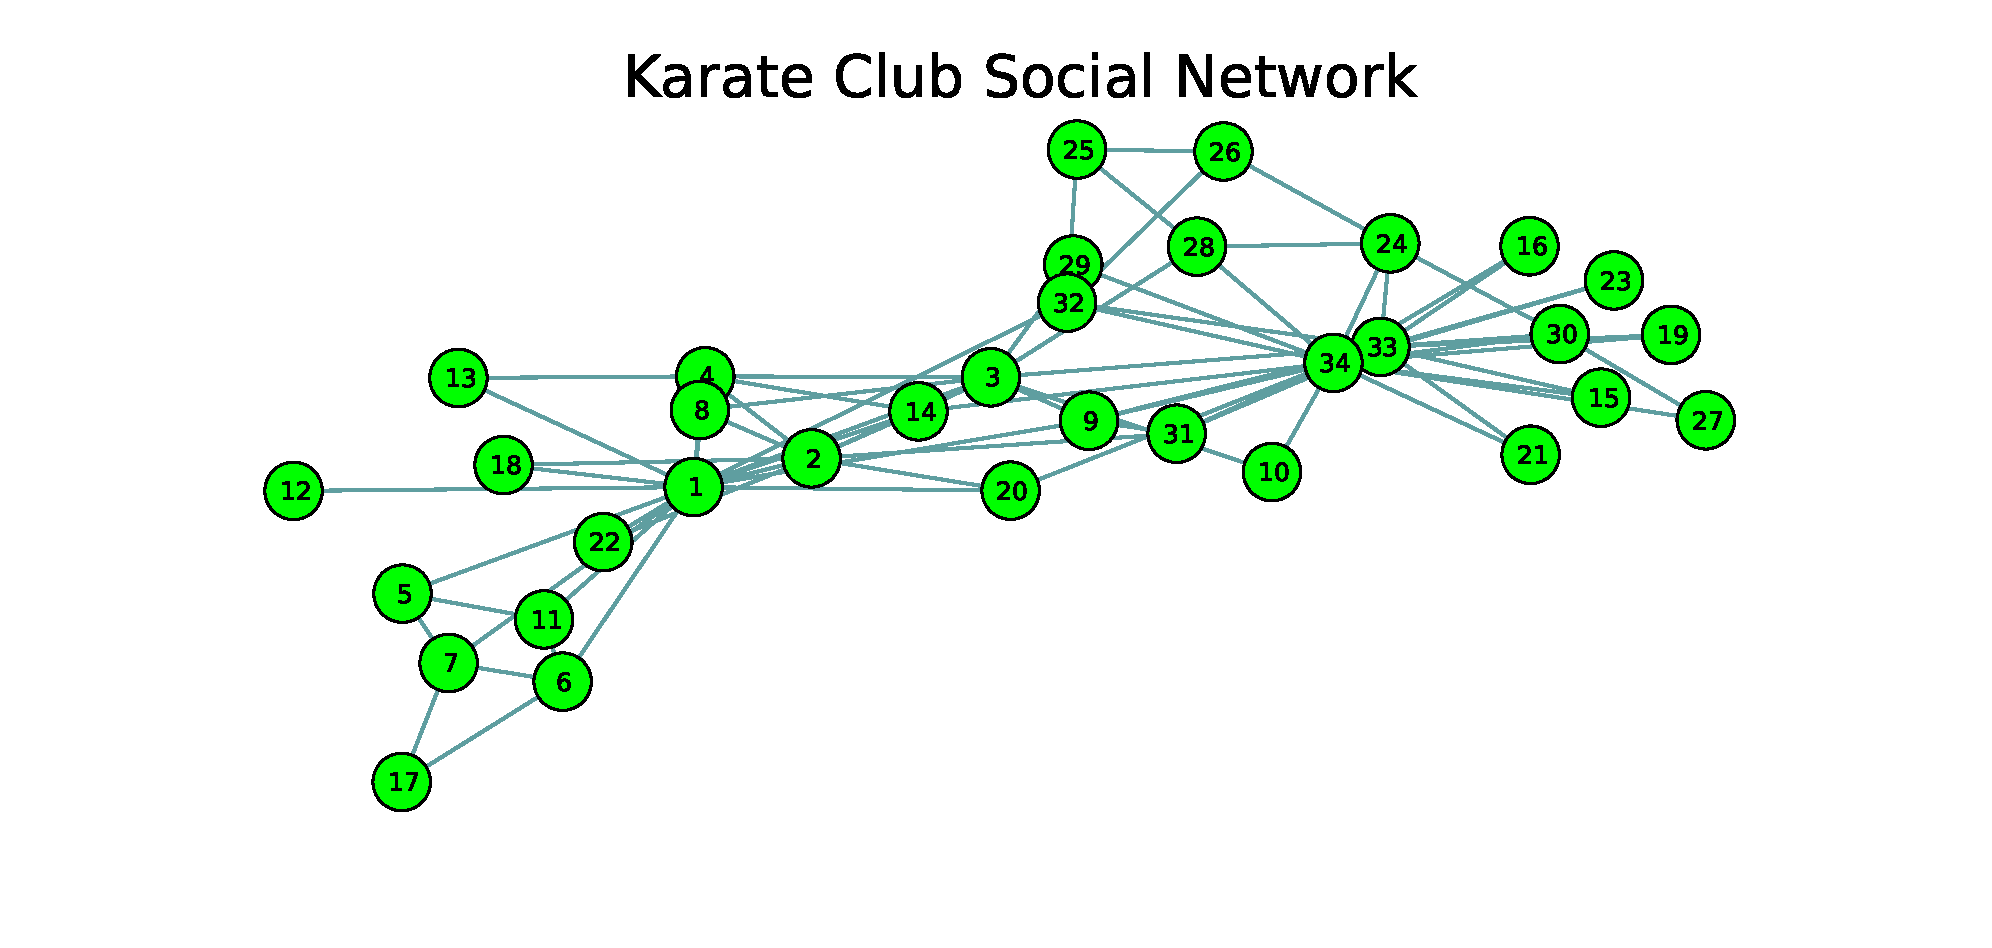
\includegraphics[width=4.5in]{Figures/karate_social_network}
\caption{Nodes are students.  Edges are students seen outside of class together.}
\end{figure}
\end{frame}



\begin{frame}\frametitle{Karate Club}
If we know the groups people form:
\begin{itemize}
\item If students disagree, who will disagree with who?
\item How many groups is someone a member of?
\item Who are the influential members of a group?
\end{itemize}
\begin{figure}
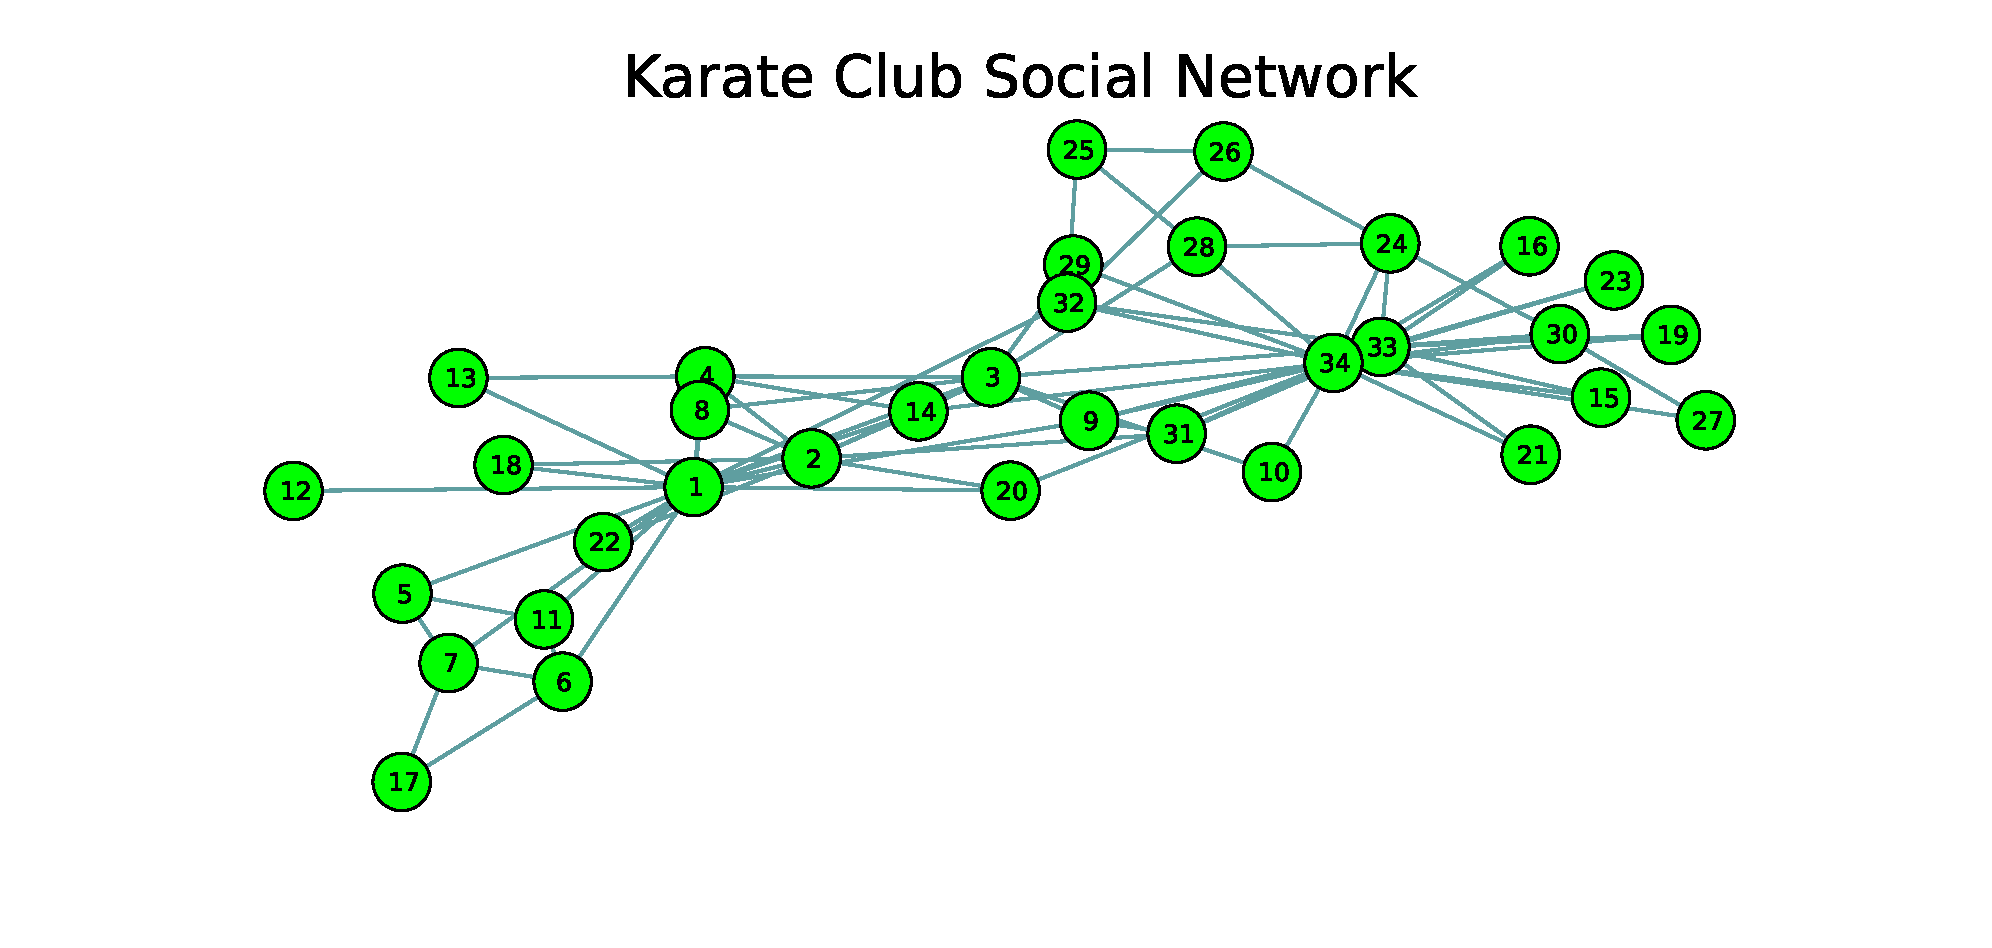
\includegraphics[width=3in]{Figures/karate_social_network}
\end{figure}
\end{frame}



\begin{frame}\frametitle{Science on Networks}

Many fields of applications have developed their own methods.

\begin{table}[!h]
\centering
\begin{tabular}{l|l}
Application & Community Detection Method \\ \hline
Computation Distribution & Recursive Bi-section [Karypis \& Kumar] \\
Statistical Mechanics & Belief Propogation [Hastings]\\
PageRank & Local Spectral Analysis [Andersen \& Chung] \\
Taxonomy & Neighbor Joining [Saitou \& Nei] \\
$\vdots$ & $\vdots$
\end{tabular}
\end{table}

\begin{block}{}
\begin{center}
How do we compare them?
\end{center}
\end{block}
Experimental comparisons have been made for certain networks.

\end{frame}



\begin{frame}\frametitle{Size of Networks}
Applications are increasing in size as they become available.

\begin{table}[!h]
\centering
\begin{tabular}{c|c|c}
Network & Number of Nodes & Date Available \\ \hline
Karate Club & 34 & 1970s \\
Astrophysics Co-authors & 19k & 1999 \\
Twitter & 20 million & 2009\\
\vdots & \vdots & \vdots \\
Facebook & 1 Billion & ???
\end{tabular}
\end{table}

\begin{block}{}
\begin{center}
We need a parallel method that scales.
\end{center}
\end{block}
Pioneer parallel methods are being developed.

\end{frame}



\begin{frame}\frametitle{Complexity of Communities, always increasing}
\begin{figure}
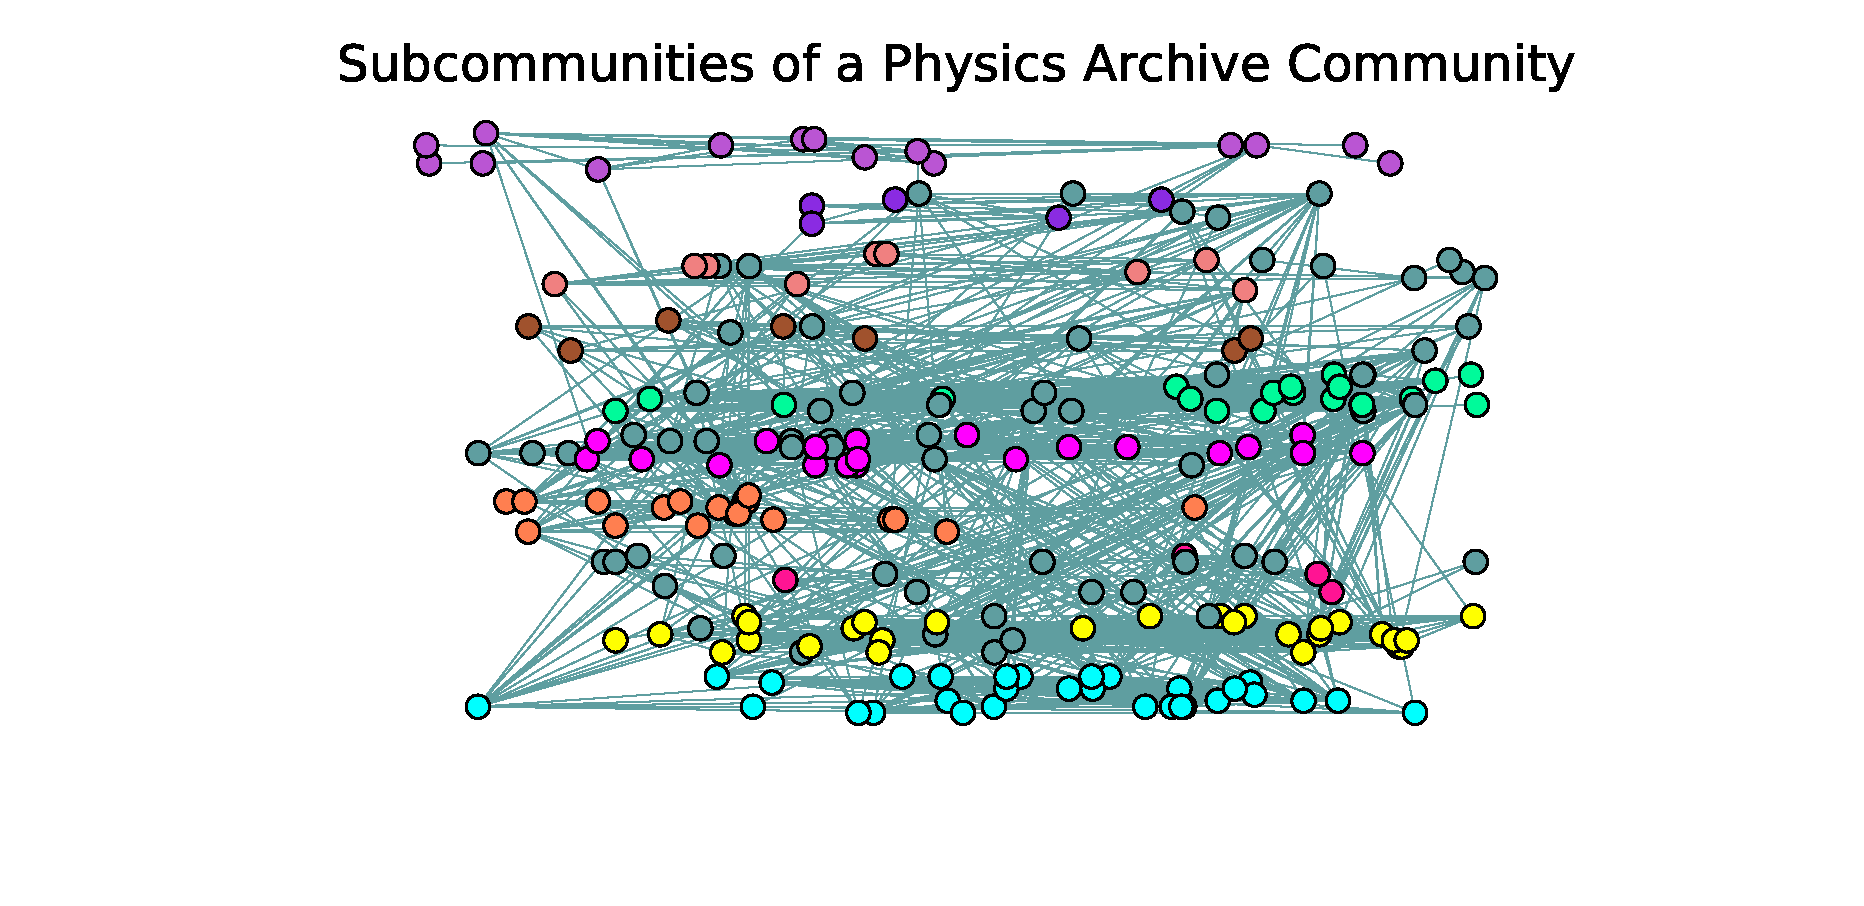
\includegraphics[width=3in]{Figures/complex}
\caption{The umbrella community is results on computing {\it flow equations}.  The subcommunities are different approaches to calculating the equations.}
\end{figure}
\begin{block}{}
\begin{center}
We need a method for weighted networks and overlapping communities.
\end{center}
\end{block}
Only predictably overlapping communities have been found.
\end{frame}


\begin{frame}\frametitle{This Talk}
\begin{center}
\begin{itemize}
\item Framework to understand Community Detection Methods. \newline
\item Parallel method for large complex networks. \newline
\item Demonstrate power of new method on: \newline
	\begin{itemize}
		\item Wikipedia Elections \newline
		\item Physics Archive Citation Network
	\end{itemize}
\end{itemize}
\end{center}

\end{frame}


\section{Framework for Understanding Methods}


\begin{frame}\frametitle{Brief Terminology}

\begin{definition}[Internal Edges]
Edges between members of the same community.
\end{definition}
\begin{figure}
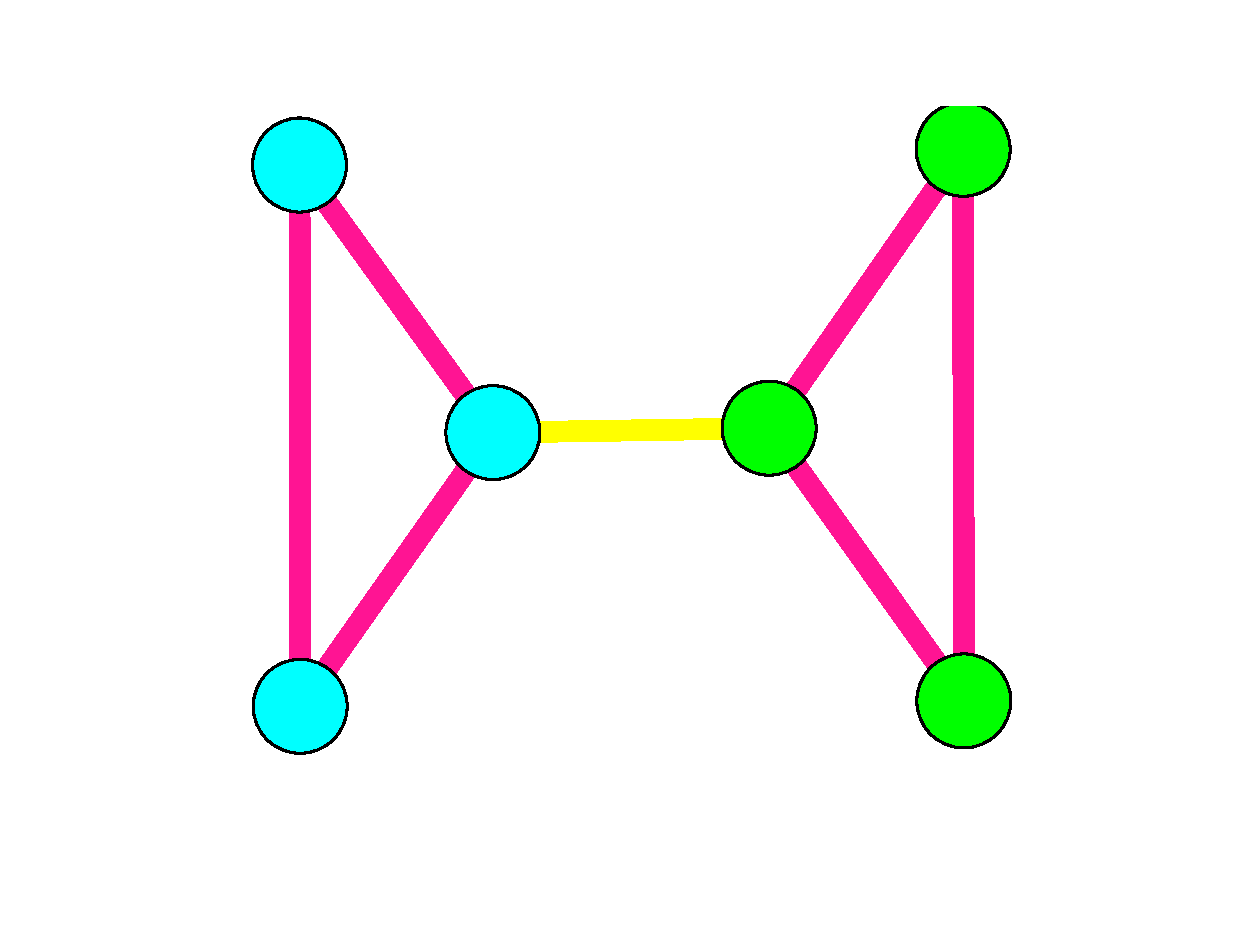
\includegraphics[width=1.5in]{Figures/int_ext_edges_graph}
\caption{Internal Edges are in Pink, External Edges are in Yellow.}
\end{figure}
\begin{definition}[External Edges]
Edges between members of different communities.
\end{definition}
\end{frame}


\begin{frame}\frametitle{Previous Community Detection Methods}
There is no universal definition of a community.  Methods pick a definition of a Community and then find those communities.
\begin{itemize}
\item $(\alpha, \beta)$ communities, every node in $C$ is connected by at least $\beta$ internal edges, every node outside of $C$ is connected by at most $\alpha$ edges. [Mishra et al]
\item Modularity, more internal edges than expected in a random graph. [Newman]
\item Conductance, probability a step in a random walk will leave the community. [used in Andersen \& Chung]
\item Edge Betweenness, remove external edges to reveal communities. [Girvan \& Newman]
\item $\cdots$ many more
\end{itemize}

\end{frame}



\begin{frame}\frametitle{Characteristics of Single Communities}

\begin{table}[t]
\centering
\begin{tabular}{c|c}
Characteristic & Desired Value \\ \hline
 {\sc Internal Density} &  large number of internal edges \\
 {\sc External Density} & small number of external edges \\
 {\sc Size} & application specific\\
 {\sc Diameter} & short \\
{\sc Average Shortest Path} & short \\
{\sc Out Degree Fraction} & small \\
{\sc Degree Distribution} & application specific \\ 
$\vdots$ &
\end{tabular}
\end{table}

\begin{block}{Representative Characteristics}
\begin{center}
All of the listed characteristics of community $C$ can be bounded by {\sc Internal Density}, $I(C)$, {\sc External Density}, $E(C)$, and {\sc Size}, $k$.
\end{center}
\end{block}
\end{frame}


\begin{frame}\frametitle{Metrics}

Metrics collapse all characteristics of a community, $C$, down to a real number.
\begin{definition}[Metric for a Single Community]
\begin{equation}
 M : \{C \in Communities\} \rightarrow \mathbb{R}\nonumber
\end{equation}
\end{definition}
Some metrics are only functions of internal density, external density, and size of a community. We assume continuity.
\begin{definition}[Metric for a Single Community]
\begin{equation}
 M : (I(C), E(C), k) \rightarrow \mathbb{R}\nonumber
\end{equation}
\end{definition}
 We can visualize how these metrics collapse the $3D$ space describing these communities to the real numbers.  We cover the dimension of size in the paper, but only consider internal density and external density here.
\end{frame}

\begin{frame}\frametitle{The 3D space of Communities}
Consider the set of $\{ (I(C), E(C)) \in [0, 1]x[0, 1]\}$ values, such that $M(C) = m$.  This forms a level sets.  We can categorize the $(I, E)$ space with level sets.
\begin{figure}
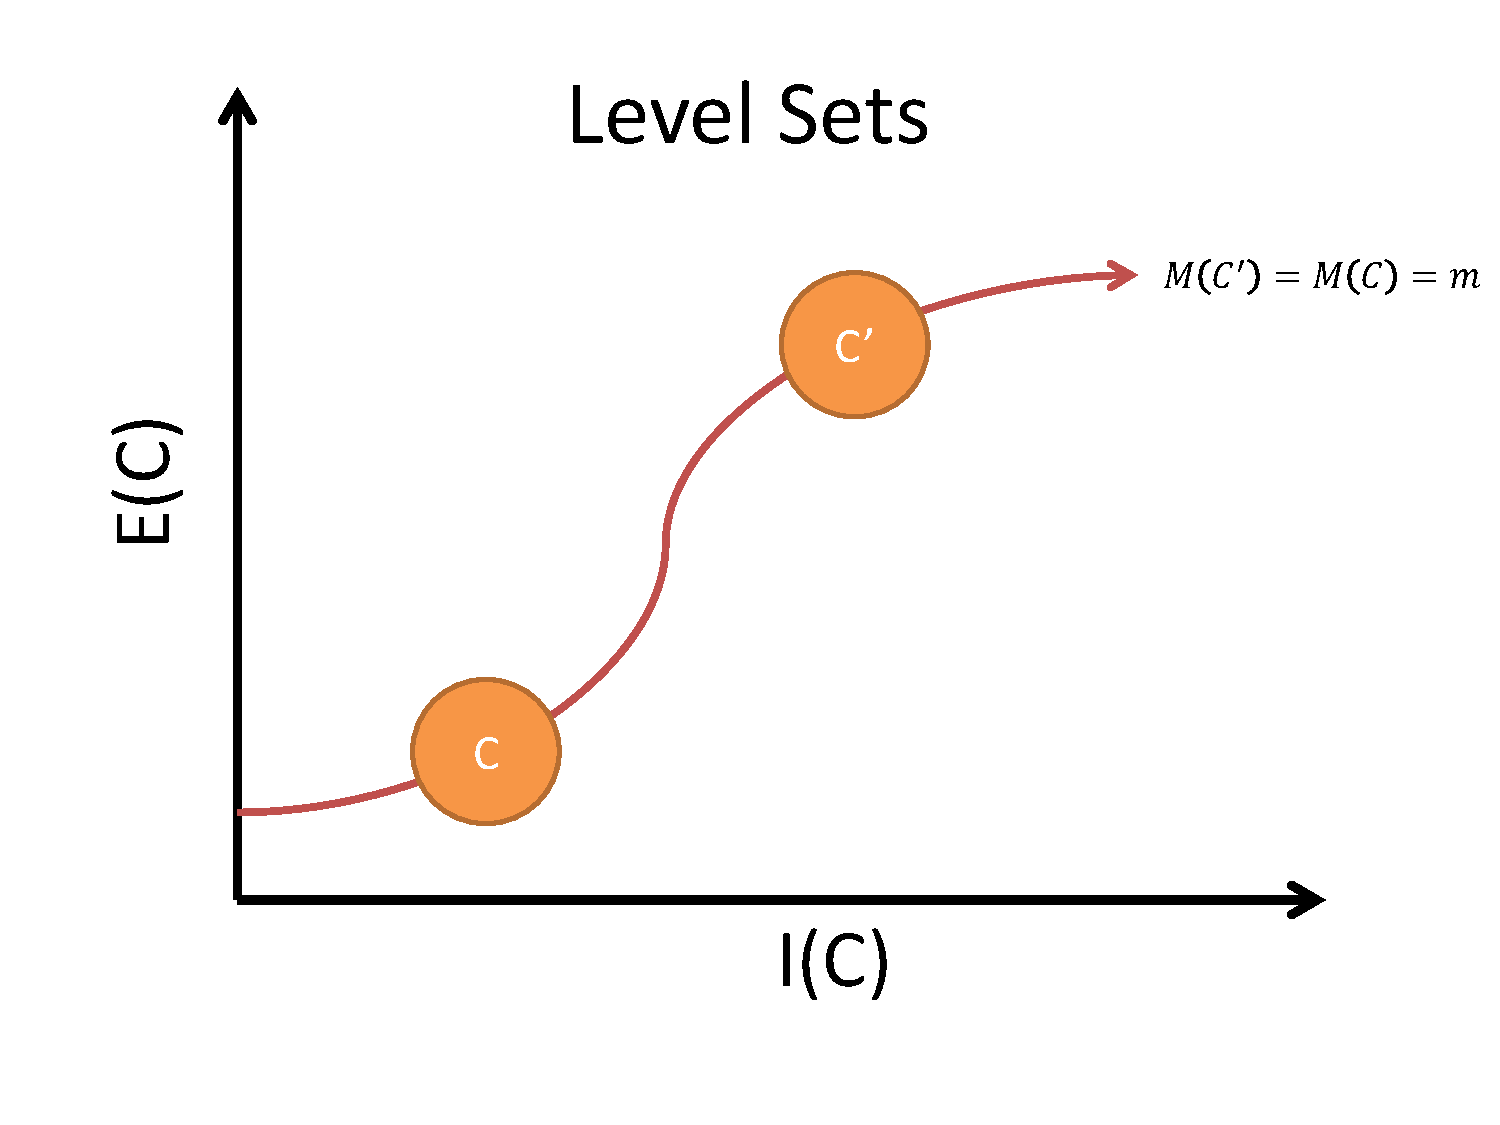
\includegraphics[width=3in]{Figures/communities_on_ls}
\end{figure}

\end{frame}

\begin{frame}\frametitle{The 3D space of Communities}
Consider the set of $\{ (I(C), E(C)) \in [0, 1]x[0, 1]\}$ values, such that $M(C) = m$.  This forms a level sets.  We can categorize the $(I, E)$ space with level sets.
\begin{figure}
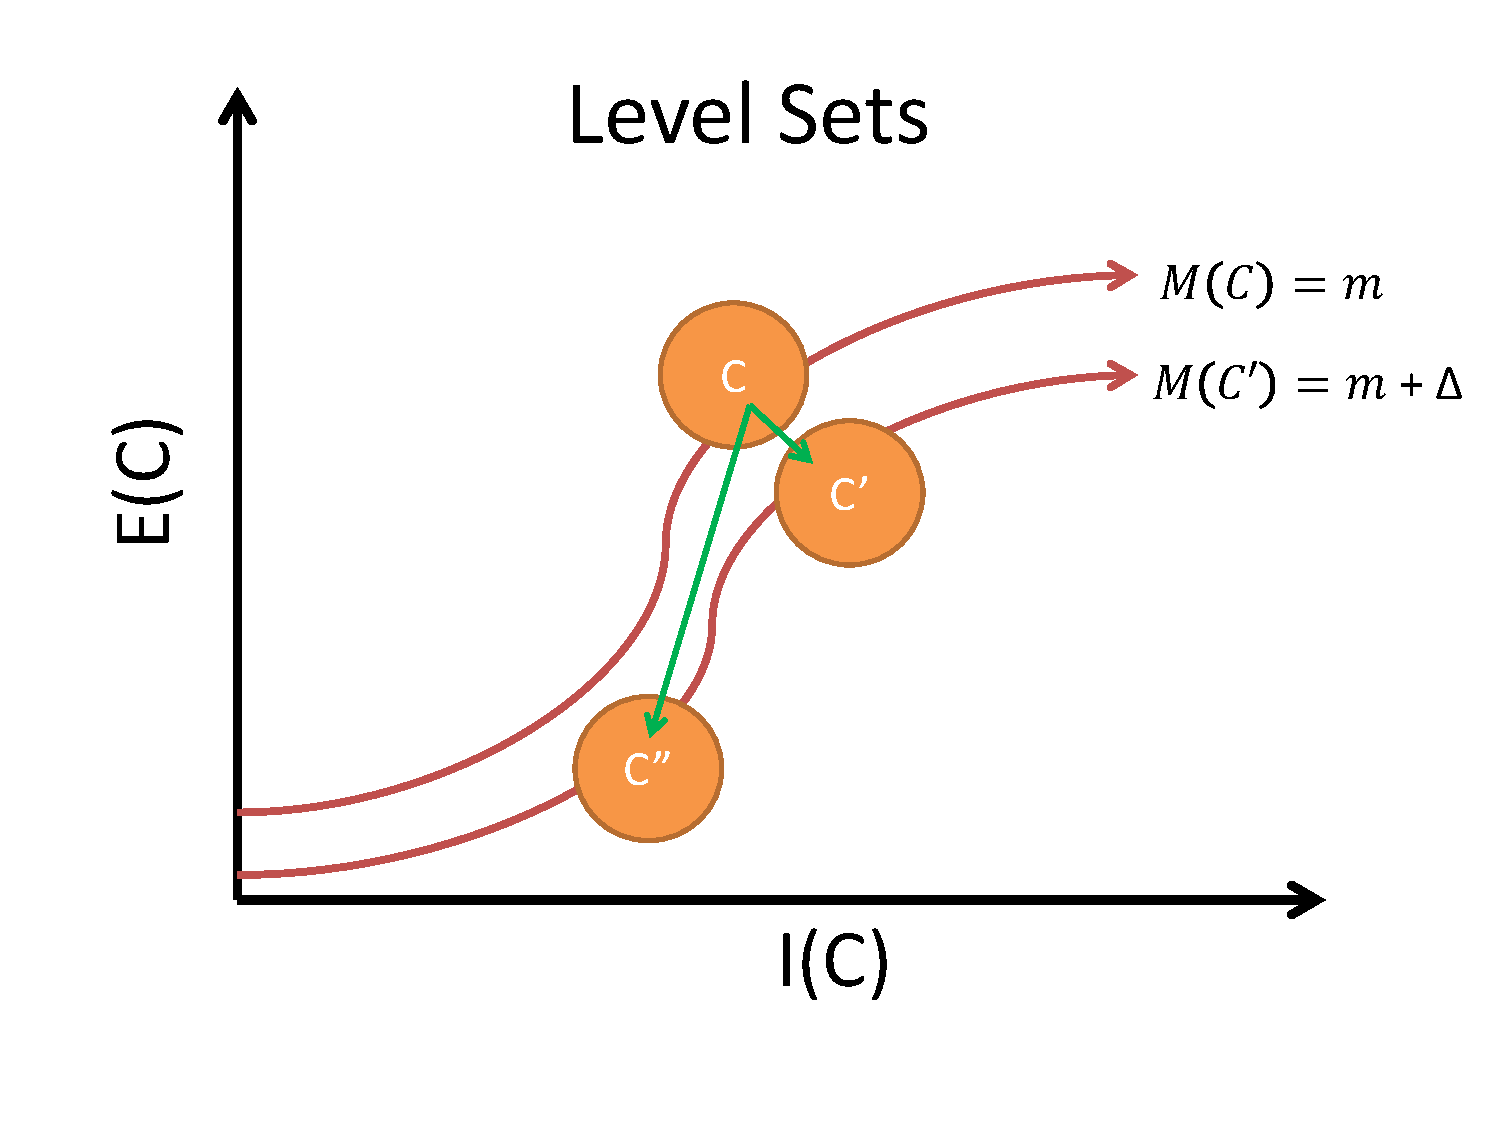
\includegraphics[width=3in]{Figures/community_change}
\end{figure}

\end{frame}



\begin{frame}\frametitle{Conductance}
Probability a random step leaves the community.
\begin{block}{}
\begin{center}
\begin{equation}
\mbox{\sc Conductance}(C) = \frac{(1 - k)E(C)}{kI(C) + (1 - k)E(C)} \nonumber
\end{equation}
\end{center}
\end{block}
Poor $I(C)$ value $\nearrow$ 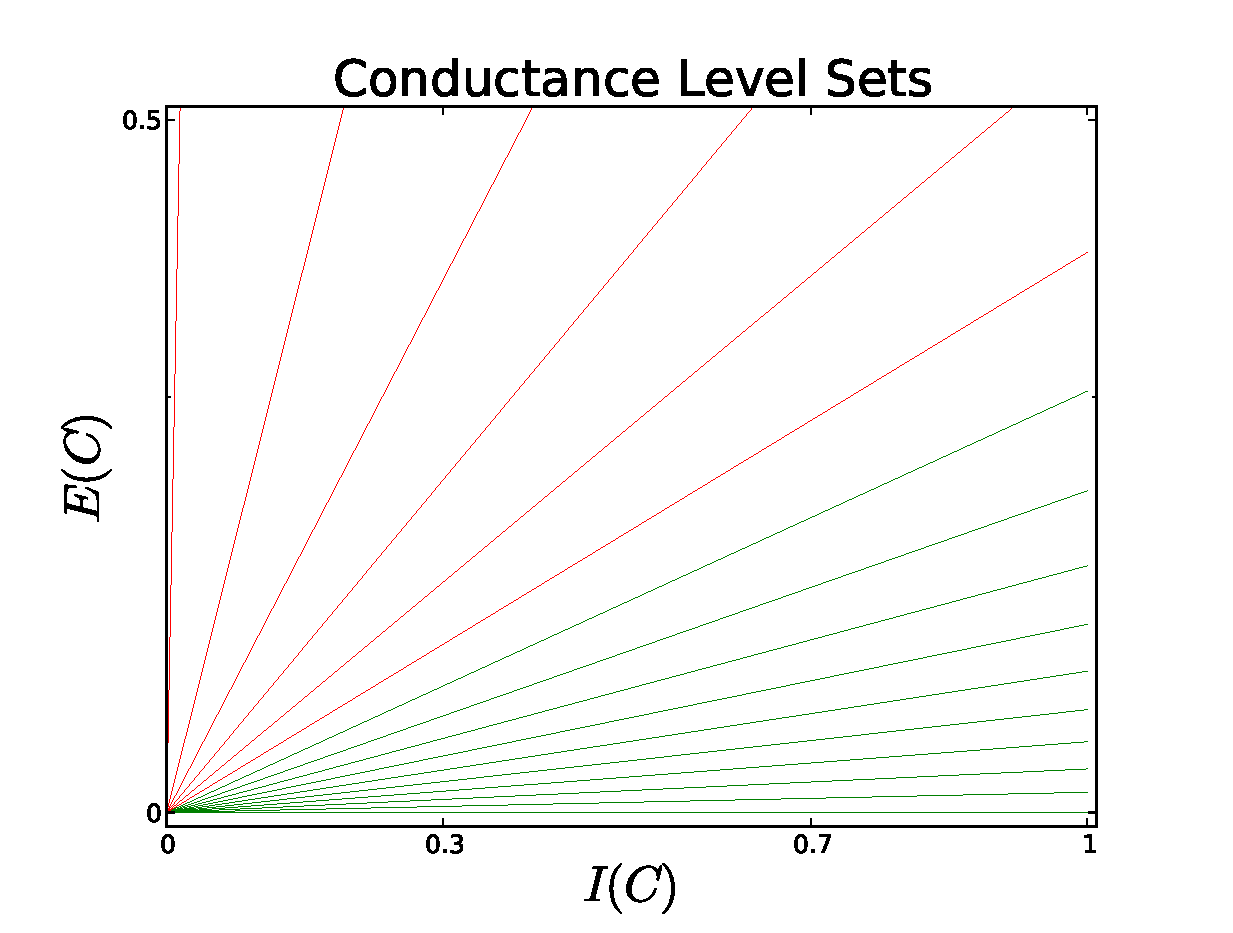
\includegraphics[width=2.5in]{Figures/cond_ls} $\nwarrow$ Good $I(C)$

\end{frame}



\begin{frame}\frametitle{Conductance}
A series of communities created by including nodes that improve conductance.

\begin{figure}
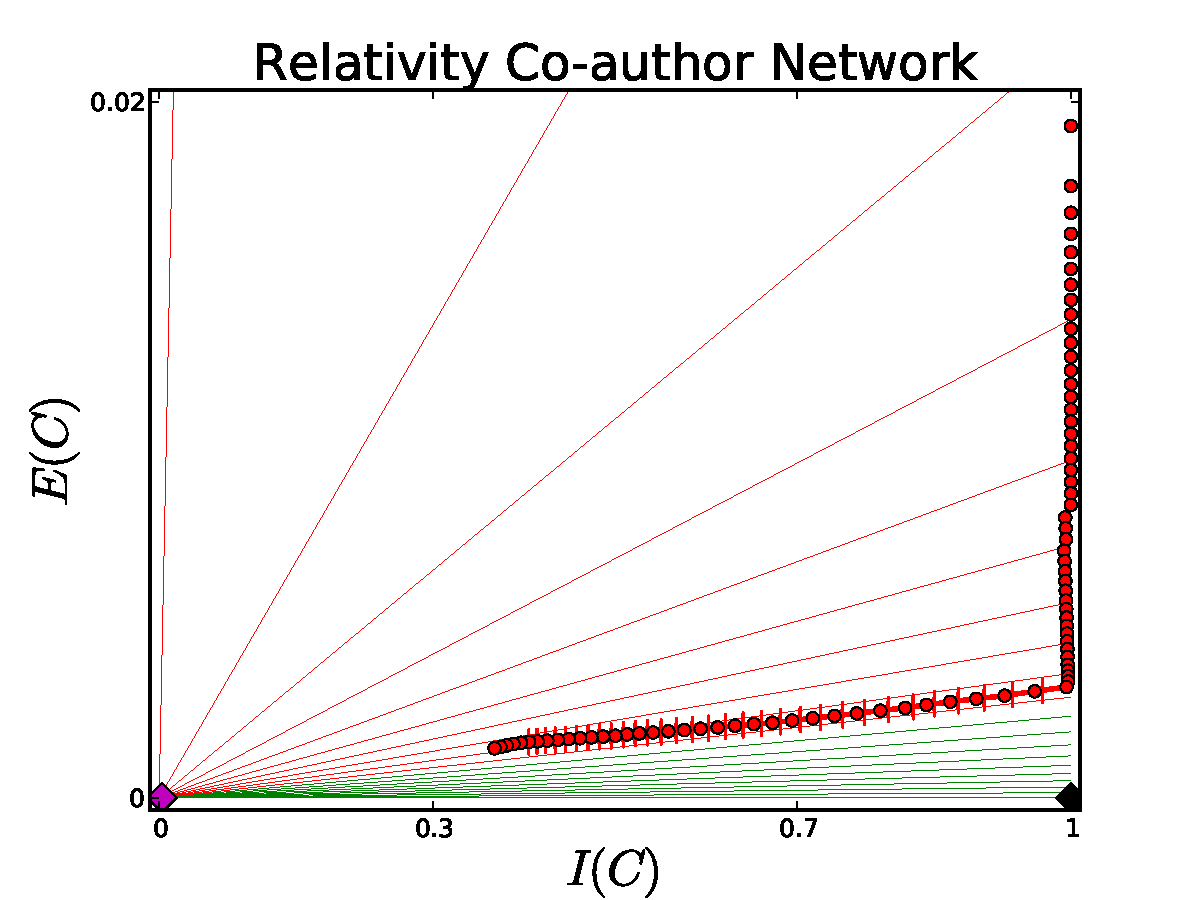
\includegraphics[width=2.2in]{Figures/conductance_relativity}
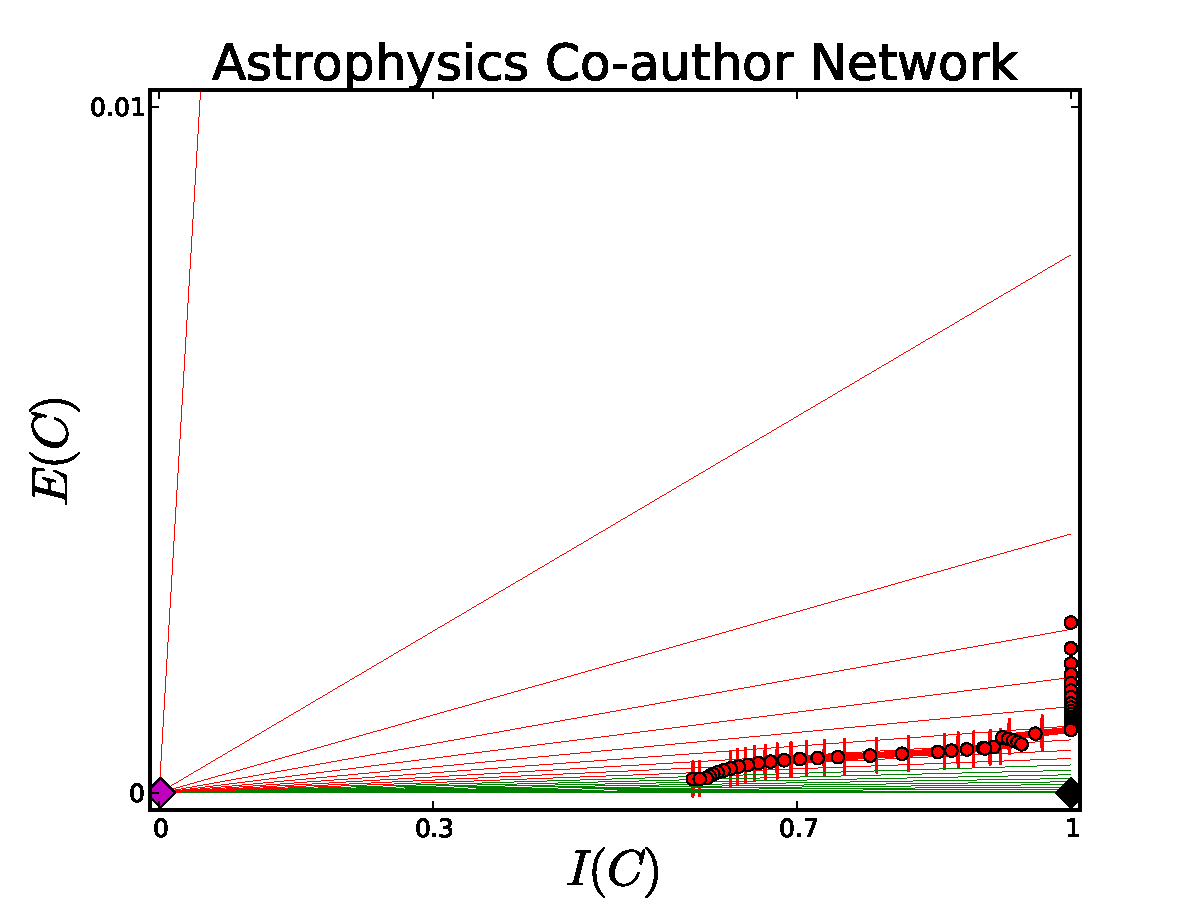
\includegraphics[width=2.2in]{Figures/conductance_astro}
\caption{The co-authors in relativity ($\approx 3k$ nodes) and astrophysics ($\approx 18k$ nodes).}
\end{figure}
Makes small improvements to external density at great cost to internal density.
\end{frame}


\begin{frame}\frametitle{Modularity of  Single Community}
Difference in present versus expected edges in a random graph.
\begin{block}{}
\begin{center}
\begin{equation}
\mbox{\sc Modularity}(C) = p I(C) - \left(p I(C) + q E(C)\right)^2.\nonumber
\end{equation}
\end{center}
\end{block}
\begin{figure}
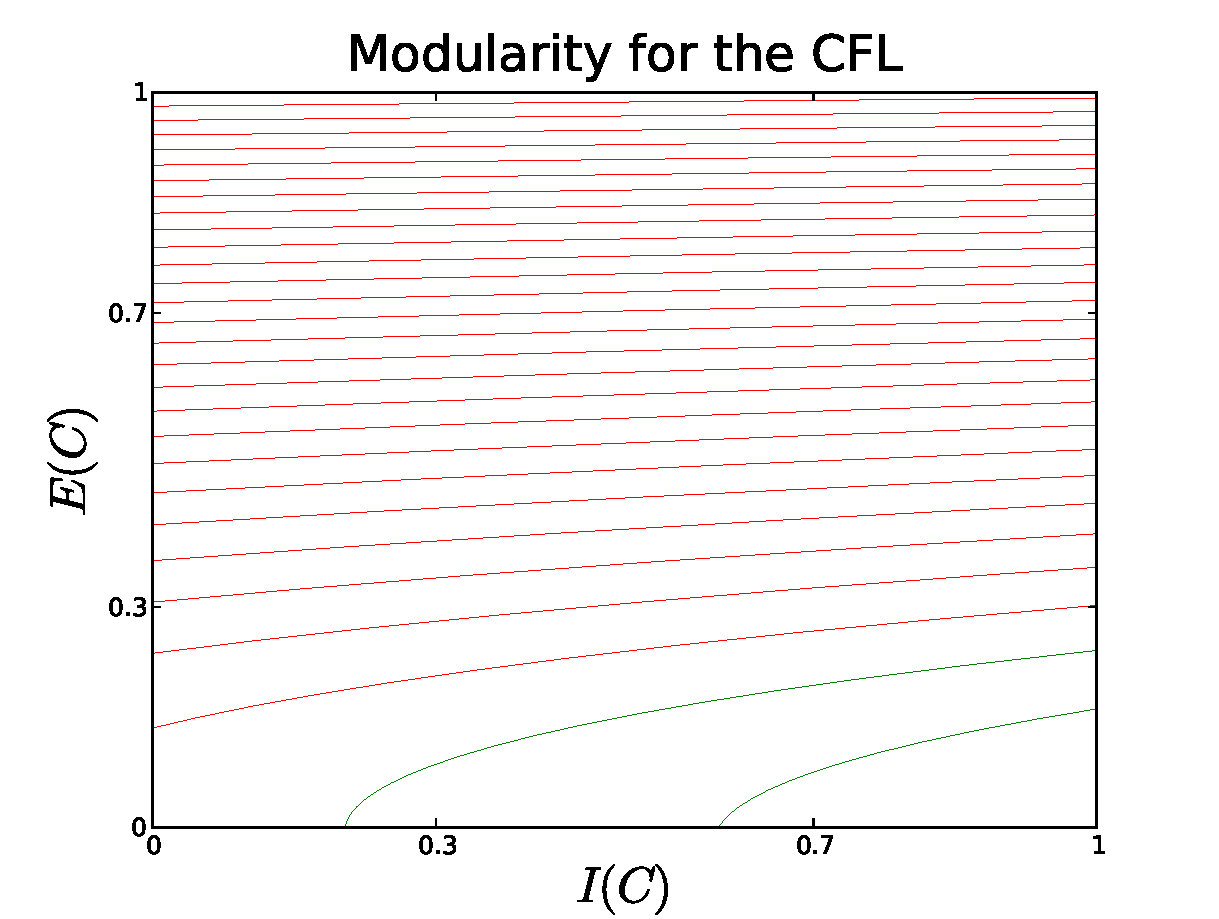
\includegraphics[width=2in]{Figures/modularity_ls}
\caption{Level Sets have the same affect as Conductance, until external density is low enough and the level sets prevent further loss in internal density.}
\end{figure}
\end{frame}



\begin{frame}\frametitle{Modularity of  Single Community}

JTODO include picture of modularity steps for a single community.

Optimizes external density and then internal density.  Optimizations of external density join together communities.  This is what causes the resolution limit in modularity.

\end{frame}

\begin{frame}\frametitle{More Single Community Metrics}

\begin{table}[t]
\centering
\begin{tabular}{p{1.5in}| p{1.5in} p{1.2in}}
Metric & definition & Results in \\ \hline
{\sc Conductance} & probability a random step leaves community & $\approx$disconnected components \\
&& \\ \hline
{\sc Edges Cut} & number edges connecting the community and graph & $\approx$disconnected components \\ && \\ \hline
{\sc Expansion} & average number of edges per node leaving the community & $\approx$disconnected components \\ && \\ \hline
{\sc Internal Density of Newman} & number of edges within a community & cliques
\end{tabular}
\end{table}

\end{frame}

\begin{frame}\frametitle{New Metric for a Single Community}

\begin{block}{}
\begin{center}
\begin{equation}
\mbox{\sc Linear}(C) = a I(C) - b E(C) \nonumber
\end{equation}
\end{center}
\end{block}
\begin{figure}
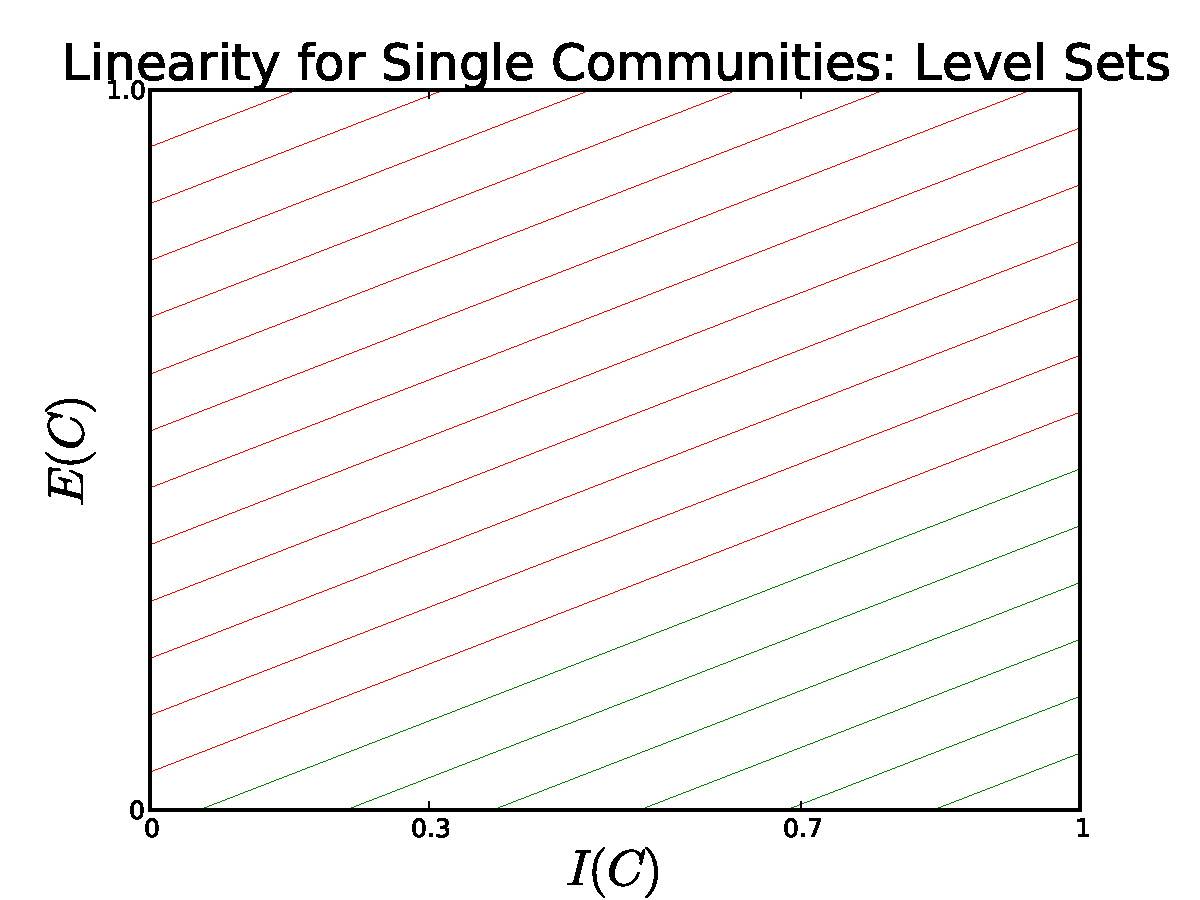
\includegraphics[width=3in]{Figures/linear_single_ls}
\end{figure}
\end{frame}


\begin{frame}\frametitle{New Metric for a Single Community}

JTODO improve
\begin{figure}
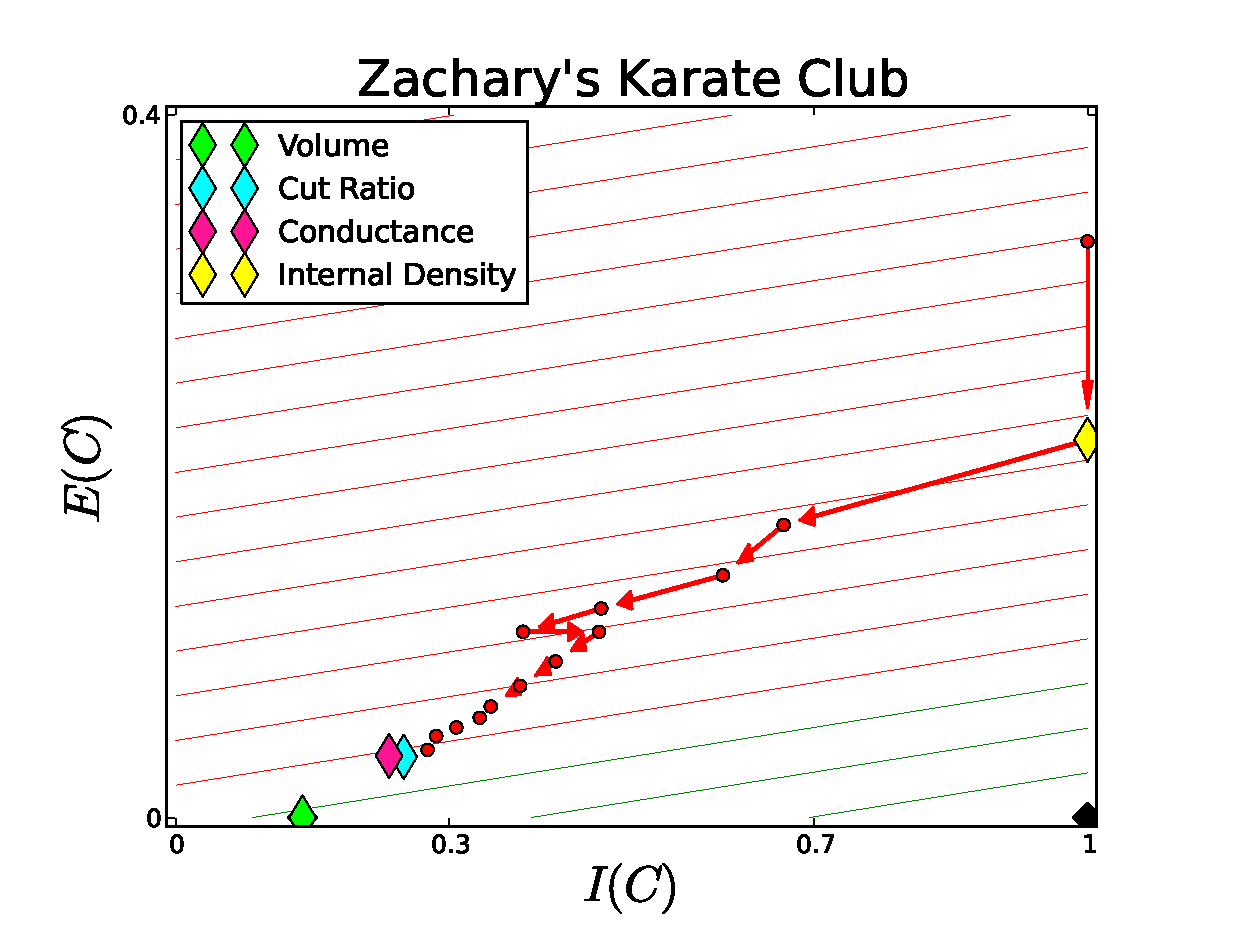
\includegraphics[width=1.5in]{Figures/linear_single_karate}
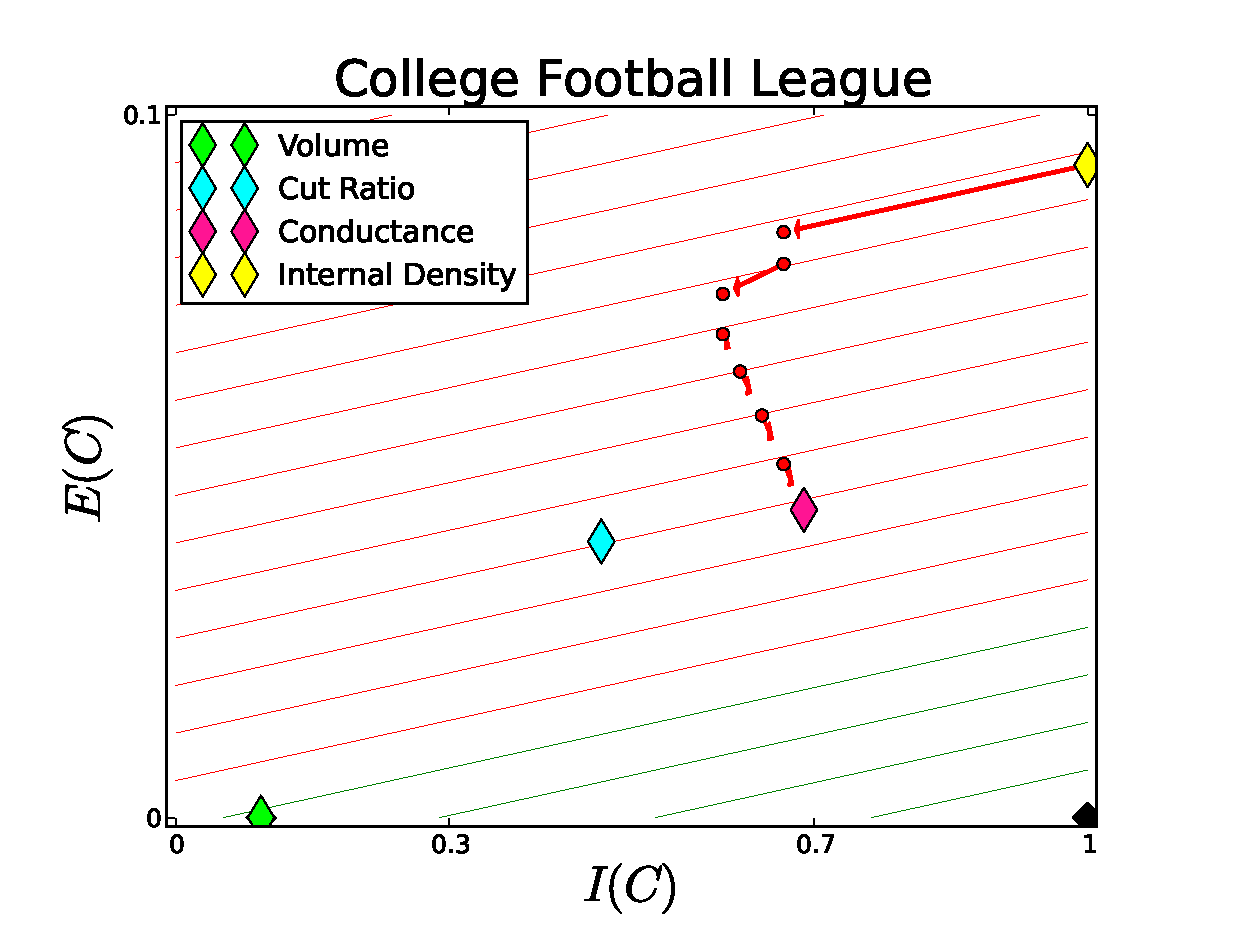
\includegraphics[width=1.5in]{Figures/linear_single_cfl}

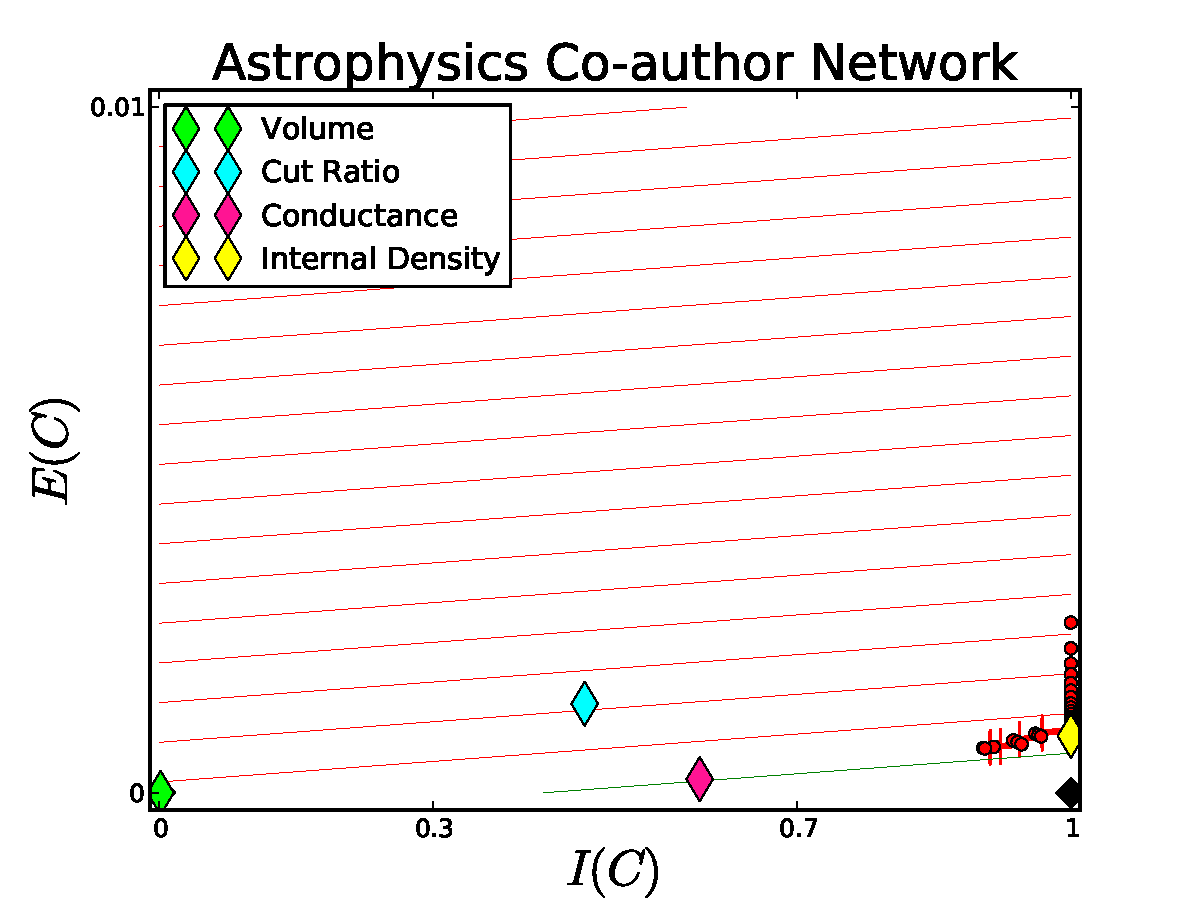
\includegraphics[width=1.5in]{Figures/linear_single_astro}
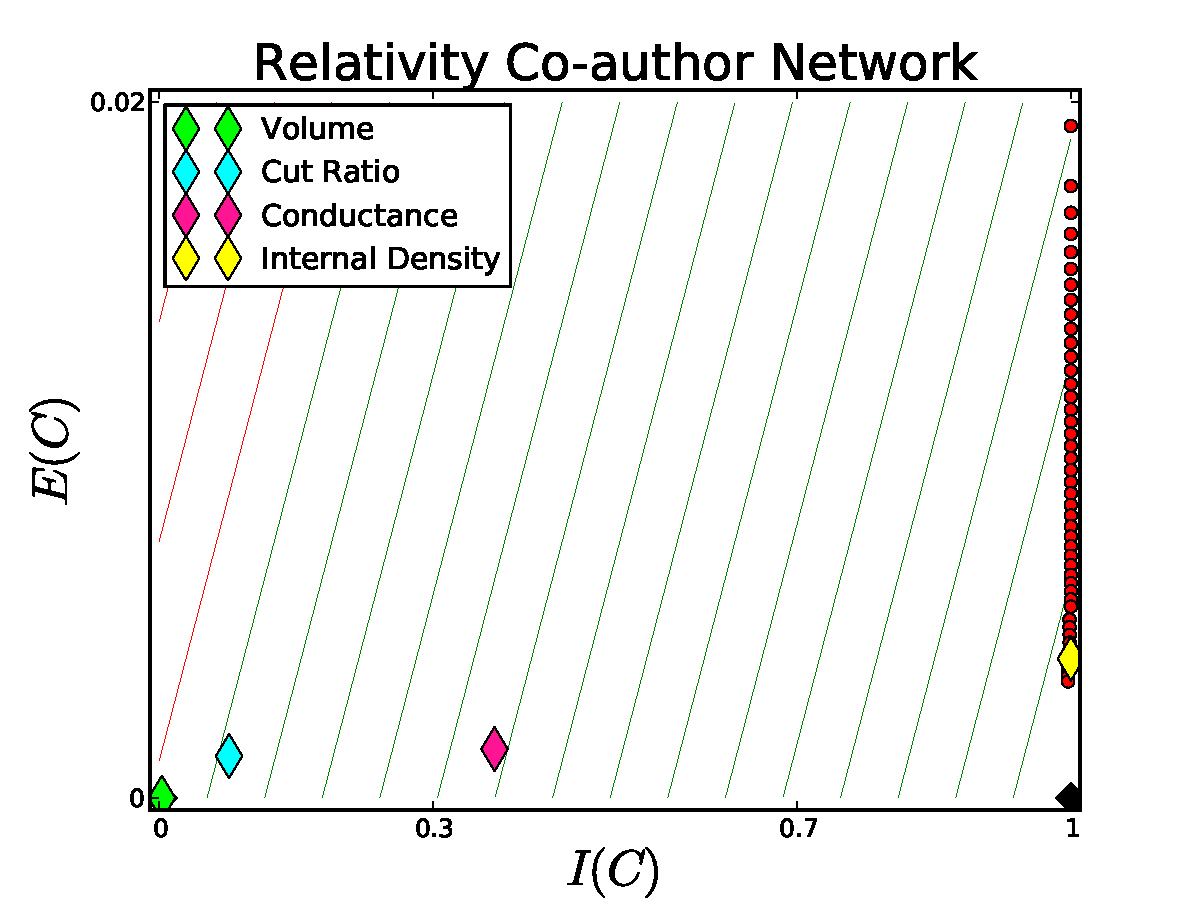
\includegraphics[width=1.5in]{Figures/linear_single_relativity}
\caption{Linear is consistently returns strong communities.}
\end{figure}
\end{frame}


\begin{frame}\frametitle{Characteristics of Sets of Communities}

Same characteristics of single communities, just adapted.

\begin{table}[t]
\centering
\begin{tabular}{c|c}
Characteristic & Represents \\ \hline
 {\sc Internal Density} &  How close communities are to cliques. \\
 {\sc External Density} & How many edges are not within a community. \\
 {\sc Size} & Number of communities.\\
 {\sc Average Diameter} &  \\
{\sc Average} $\dots$ &
\end{tabular}
\end{table}

\begin{block}{Representative Characteristics}
\begin{center}
Listed characteristics of  communities, $S = \{C_1, C_2, \dots\}$, can be bounded by {\sc Internal Density} $I(S)$, {\sc External Density} $E(S)$, and {\sc Size} $|S|$.
\end{center}
\end{block}
\end{frame}



\begin{frame}\frametitle{New Metric for a Sets of Communities}

\begin{block}{{\sc Linear}$(S)$}
\begin{center}
For constants, $a,b,c \in (0, 1)$ and set of communities $S = \{C_1, C_2, \dots \}$:
\begin{equation}
\mbox{\sc Linear}(S) = a I(S) - b E(S) - c |S| \nonumber
\end{equation}
\end{center}
\end{block}


\begin{definition}[Internal Density of a Set of Communities]
\begin{equation}
I(S) = \frac{\sum_{C \in S}  \mbox{Number of edges in } C}{\sum_{C \in S} \frac{1}{2}|C|(|C| - 1)} \nonumber
\end{equation}
\end{definition}

\begin{definition}[External Density of a Set of Communities]
\begin{equation}
E(S) = \frac{\mbox{Number of Edges not in some }C} {\mbox{Number of Edges in the Graph}} \nonumber
\end{equation}
\end{definition}

\end{frame}

\begin{frame}\frametitle{Tools For Building an Algorithm}

\begin{block}{}
\begin{center}
Can use the fast Louvain heuristic algorithm to find a partition that maximizes {\sc Linear}$(S)$.
\end{center}
\end{block}

\begin{block}{Conjecture}
\begin{center}
A greedy algorithm can ({\it almost always}) only decrease internal density.
\end{center}
\end{block}
The known exception occurs when a comparatively large clique is involved, very rare.
\end{frame}


\begin{frame}\frametitle{Greedy Algorithm for Linear}

\begin{table}[ht]
\centering
\begin{tabular}{p{1.2in} p{.05in} p{1.3in} p{.05in} p{1.3in}}
Find Cliques && Find Partition &&Expand Partitions \\
$(a,b,c) = (1, 0, 0)$ &  &  $(a, b, c)=(1, \Delta, \Delta)$ &  &  $(a, b, c)=(1, \Delta, \Delta)$\\
& $\rightarrow$ & & $\rightarrow$ & \\
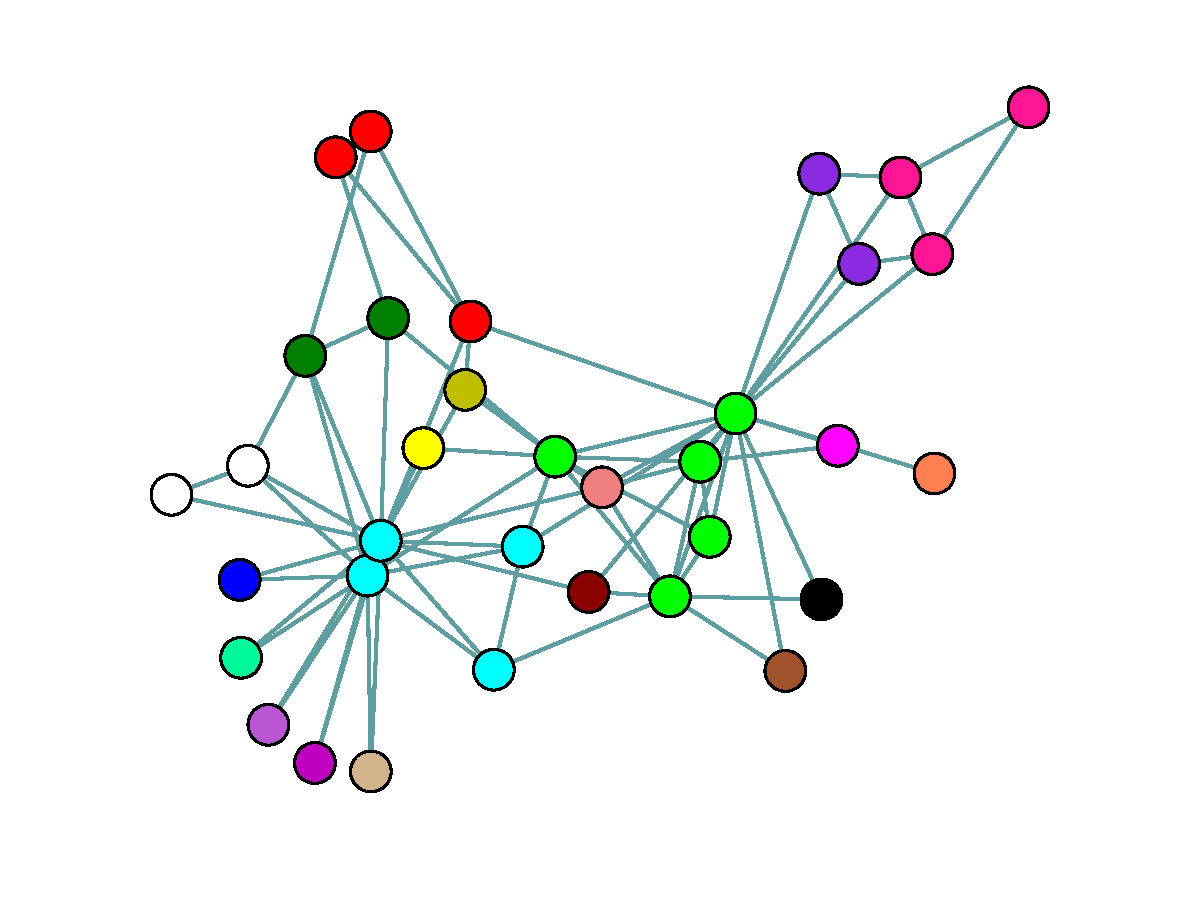
\includegraphics[width=1.5in]{Figures/clique_stage_karate} &&
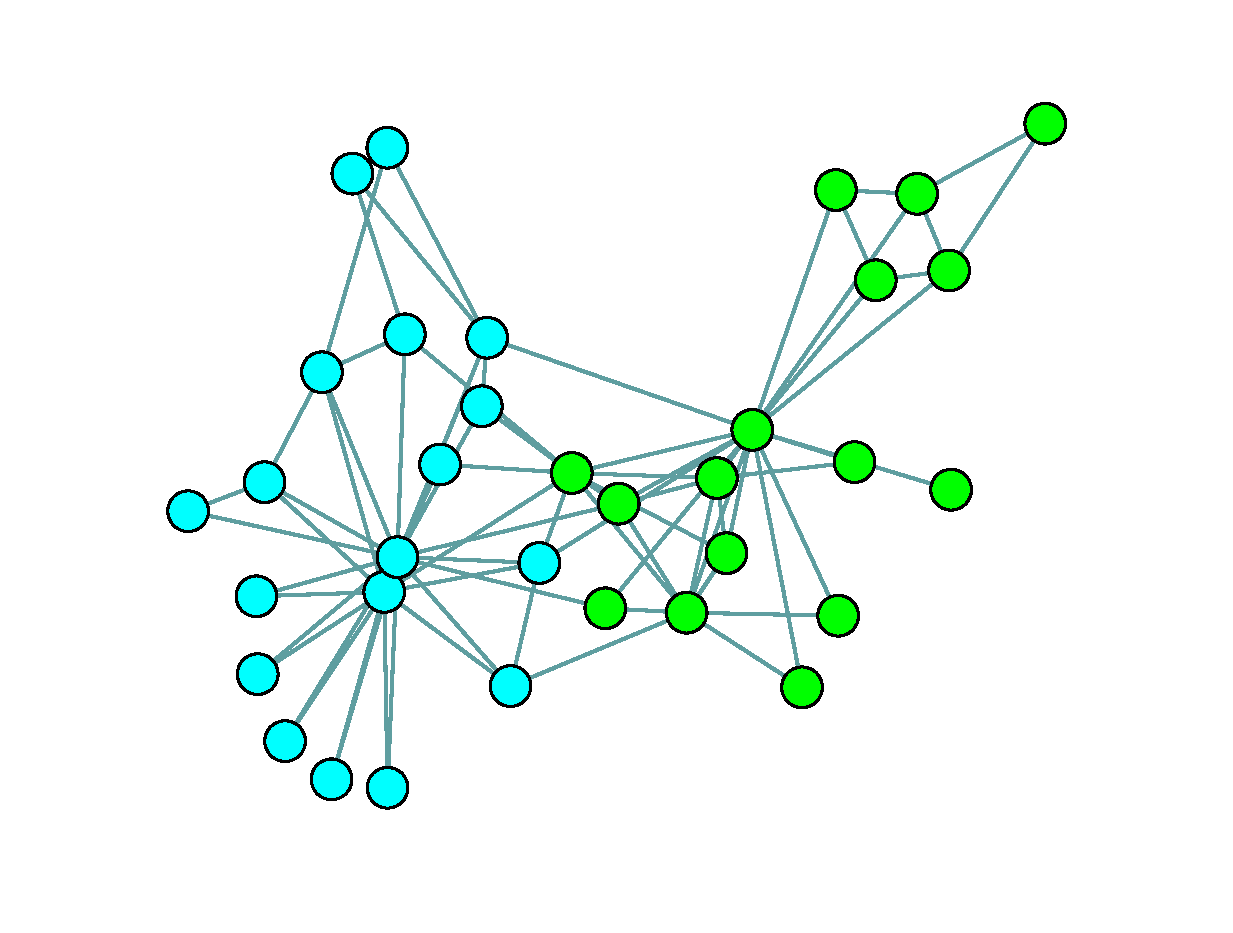
\includegraphics[width=1.5in]{Figures/partition_stage_karate} &&
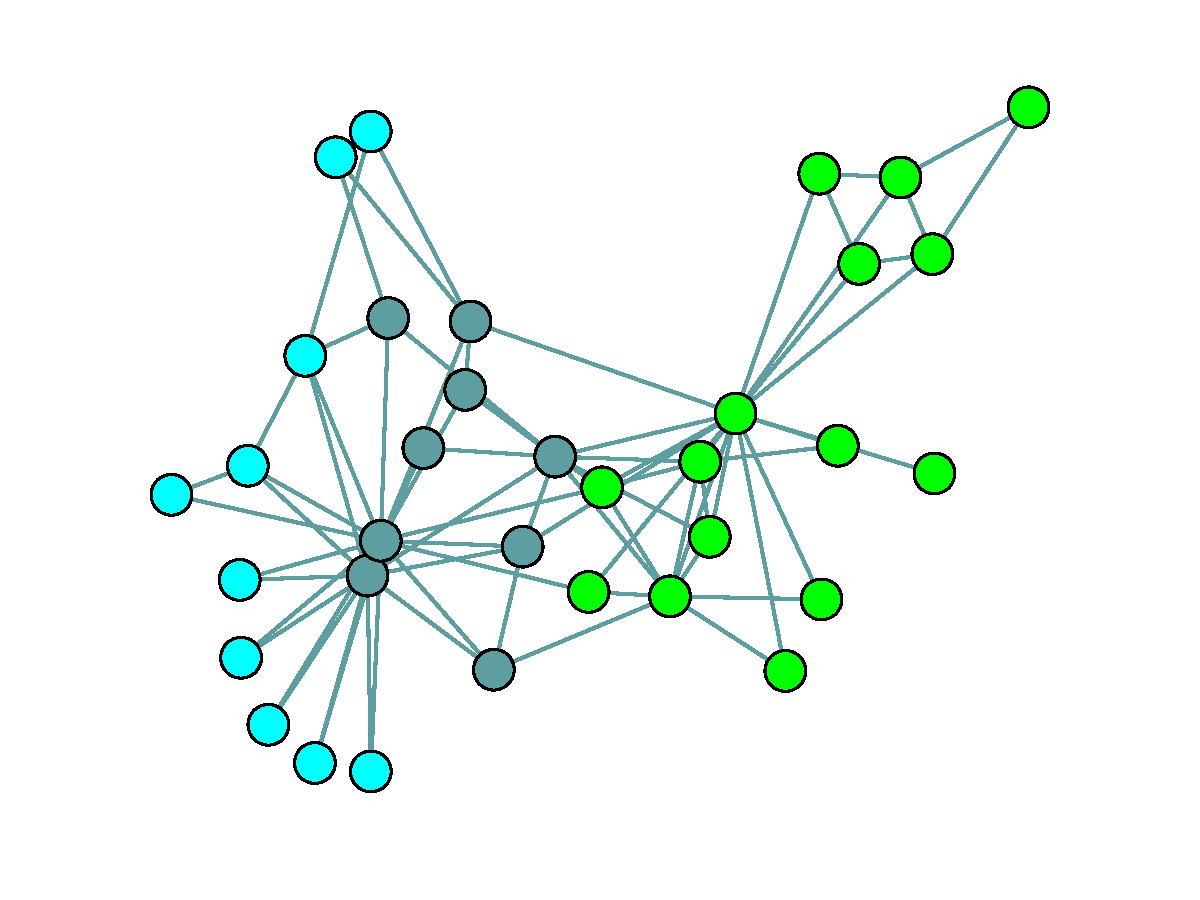
\includegraphics[width=1.5in]{Figures/expanded_stage_karate} \\
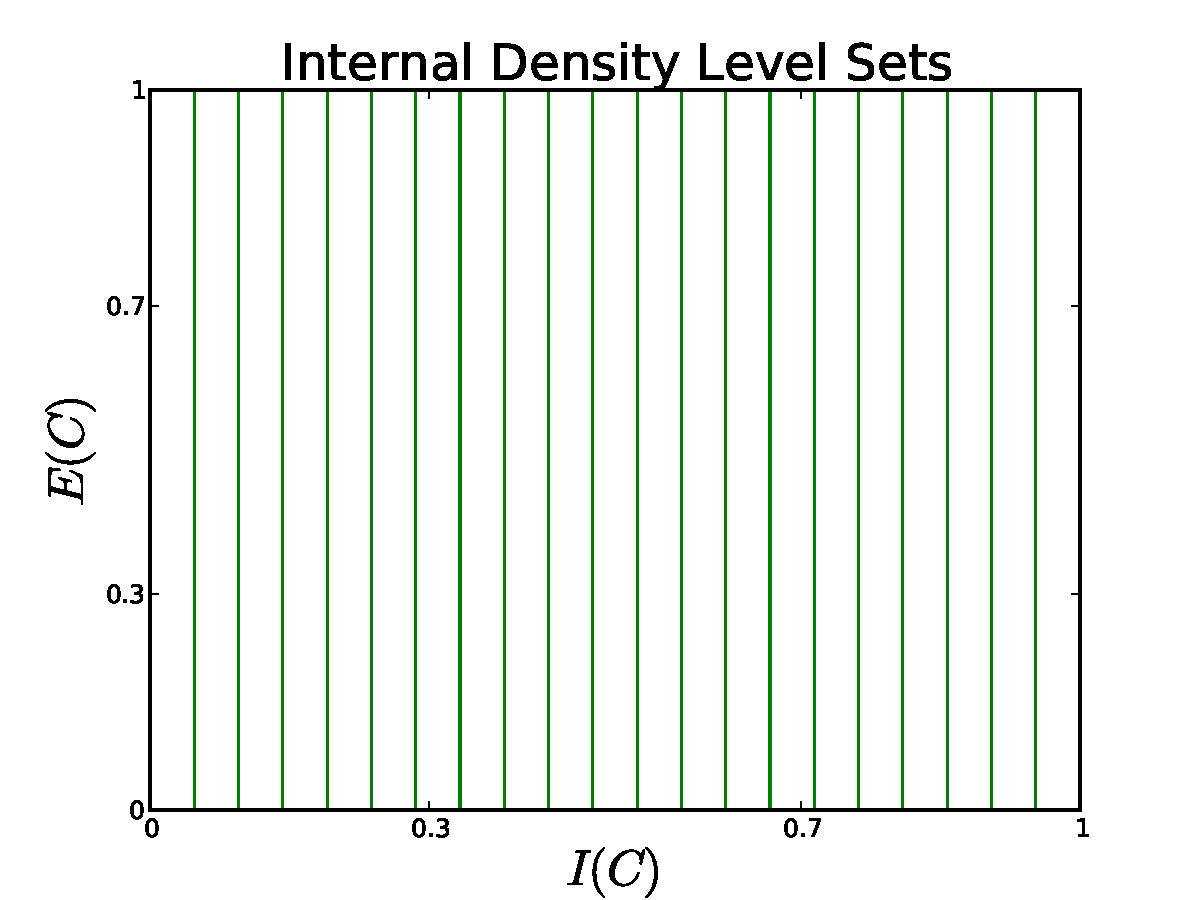
\includegraphics[width=1in]{Figures/prev_int_ls} &&
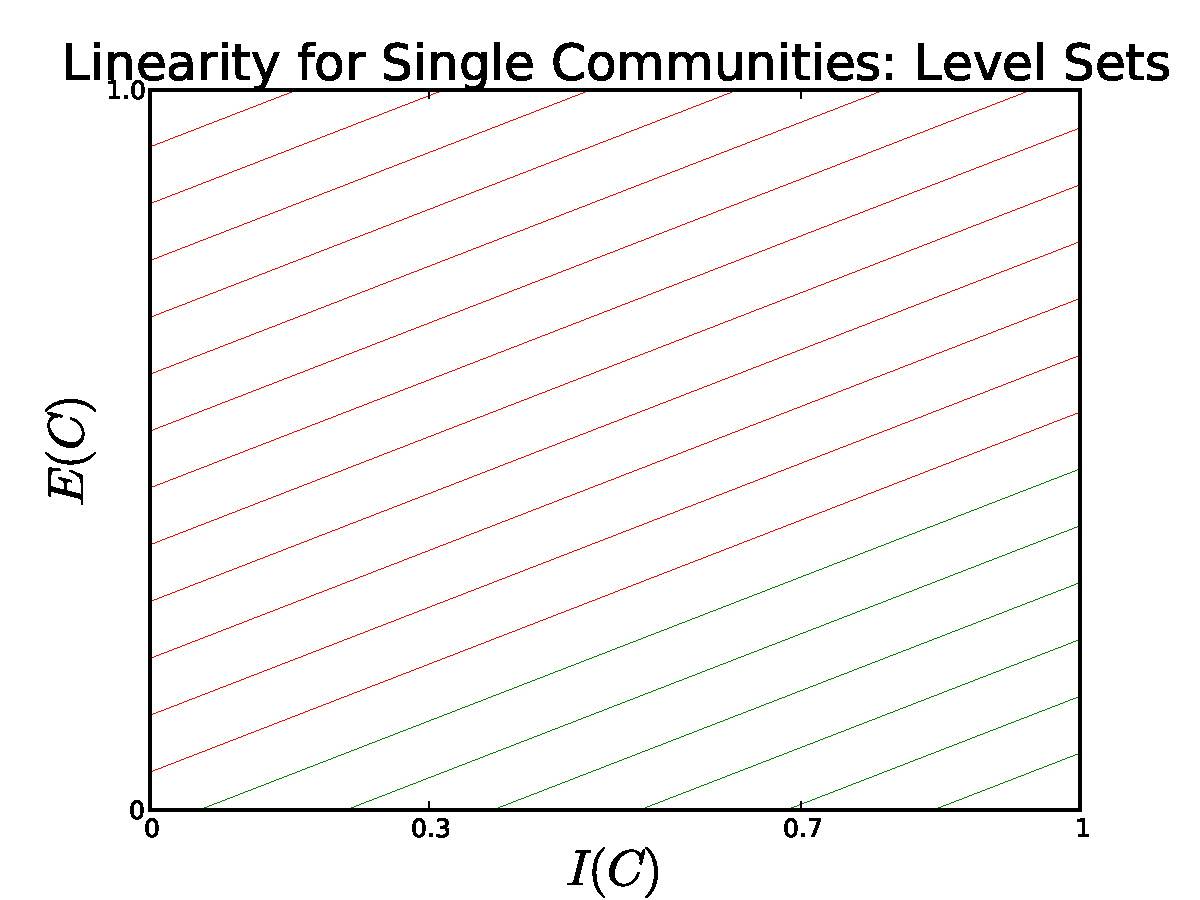
\includegraphics[width=1in]{Figures/linear_single_ls} &&
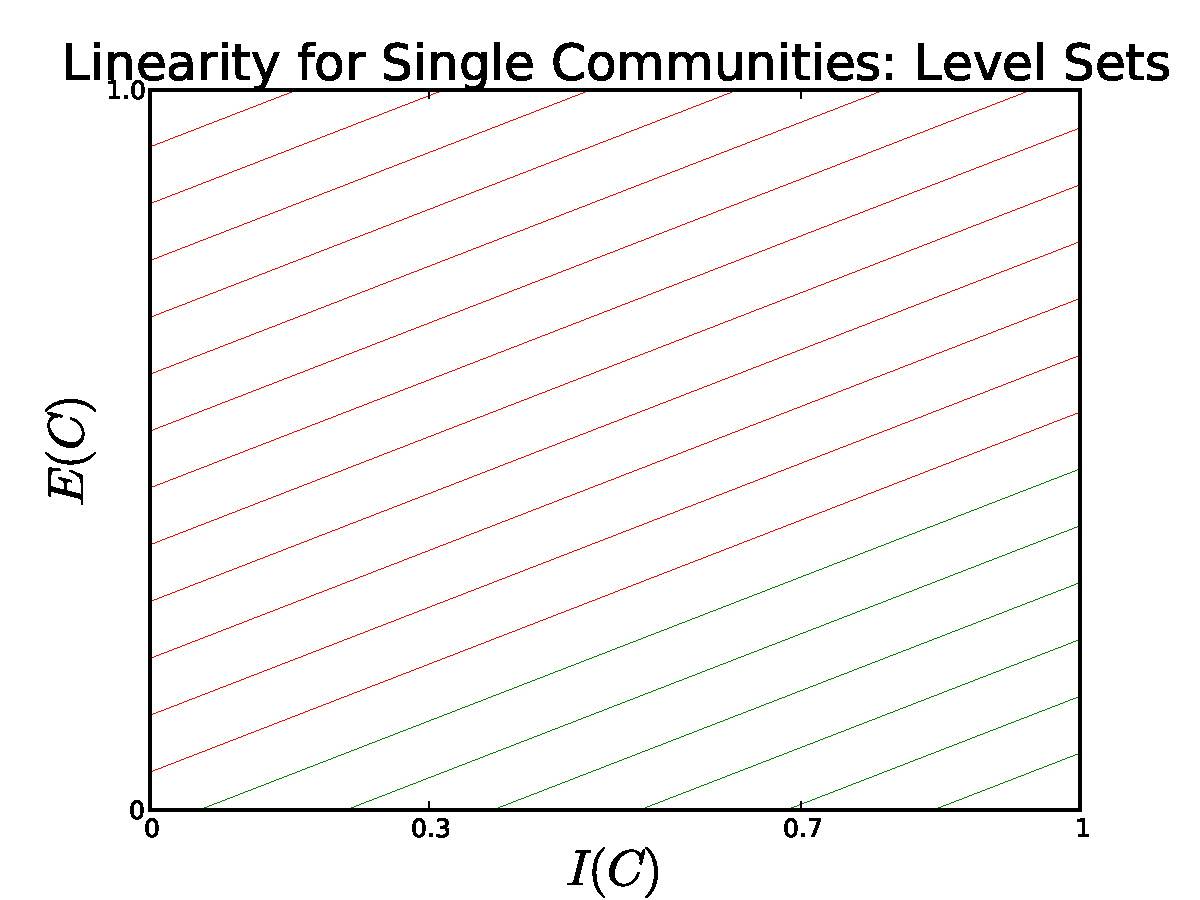
\includegraphics[width=1in]{Figures/linear_single_ls}
\end{tabular}
\caption{Communities are indicated by node color.  Nodes in multiple communities are grey.}
\end{table}

\end{frame}



\begin{frame}\frametitle{Algorithm for Linear in the IE plane}

\begin{figure}
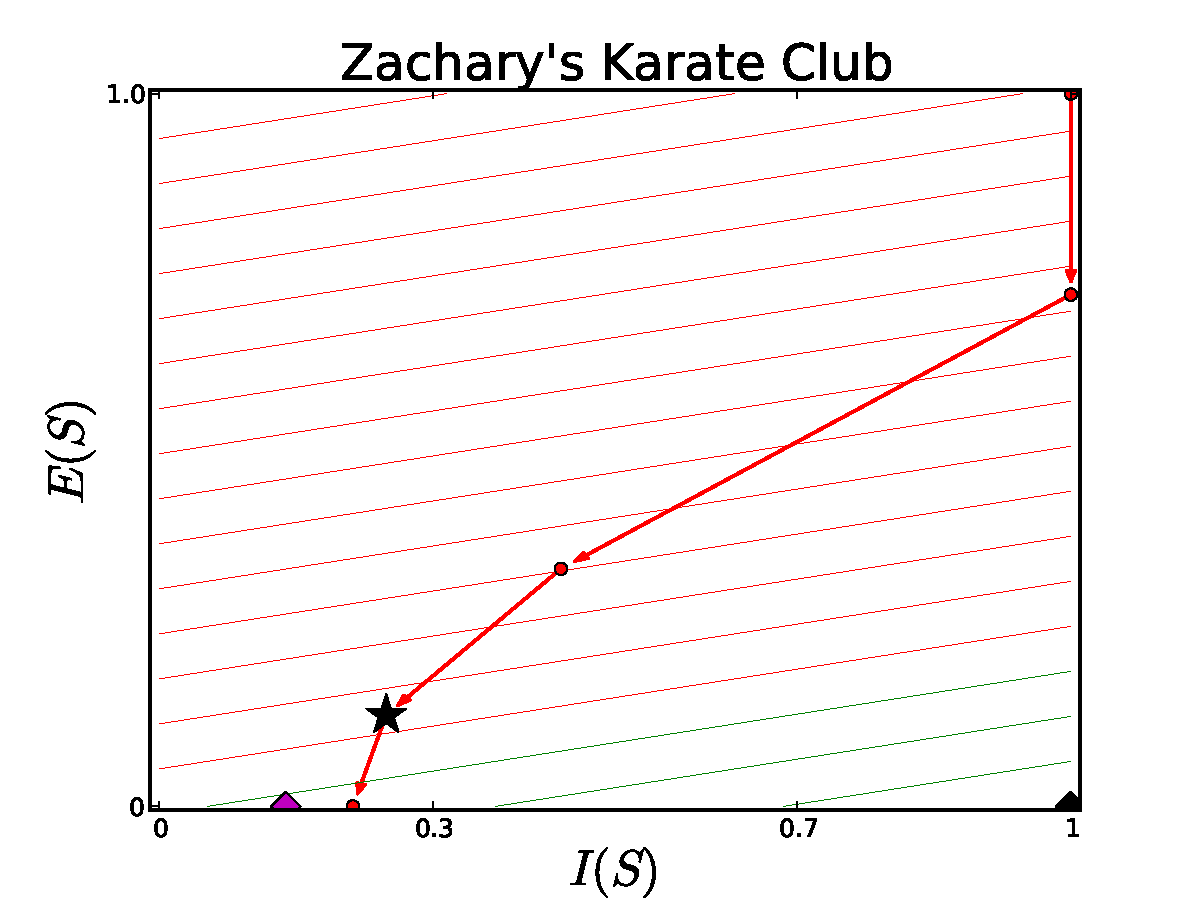
\includegraphics[width=1.5in]{Figures/linear_sets_karate}
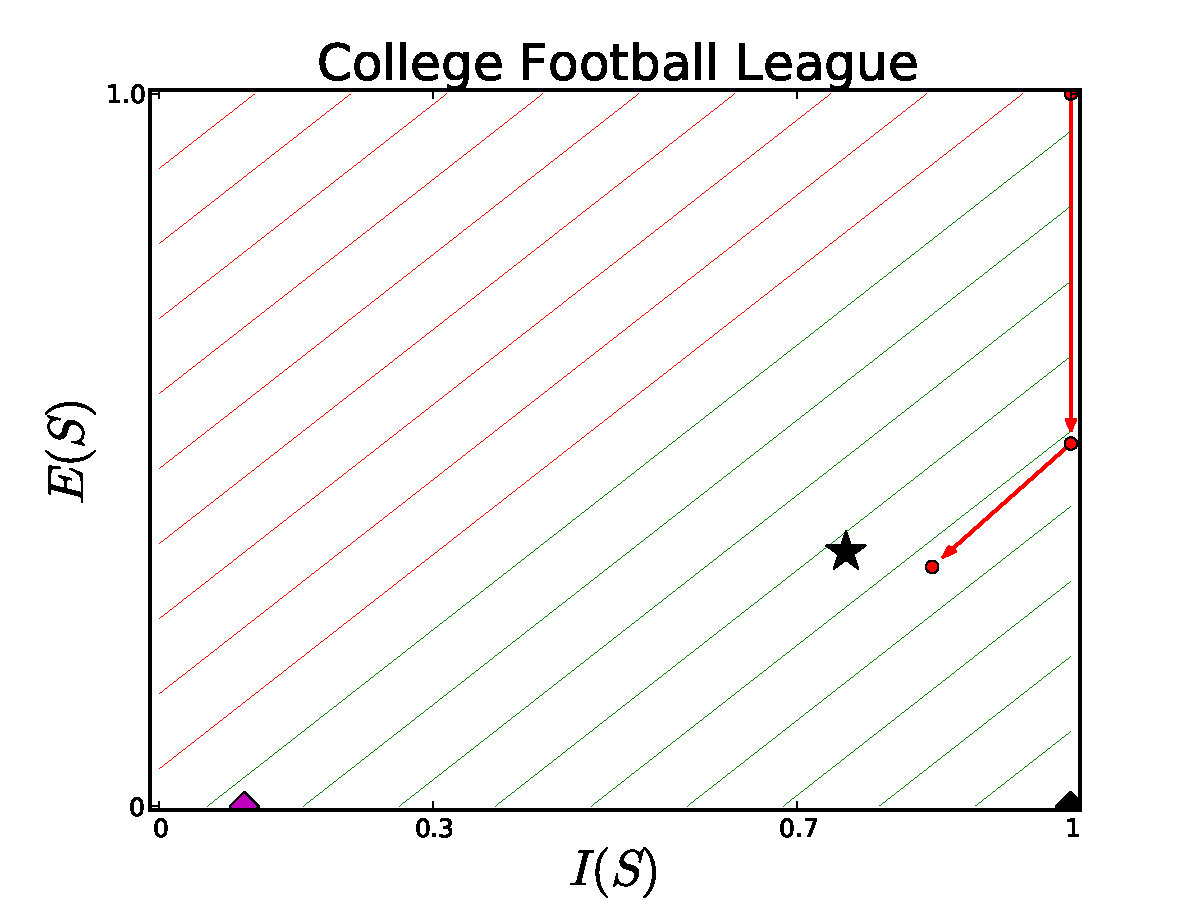
\includegraphics[width=1.5in]{Figures/linear_sets_cfl}

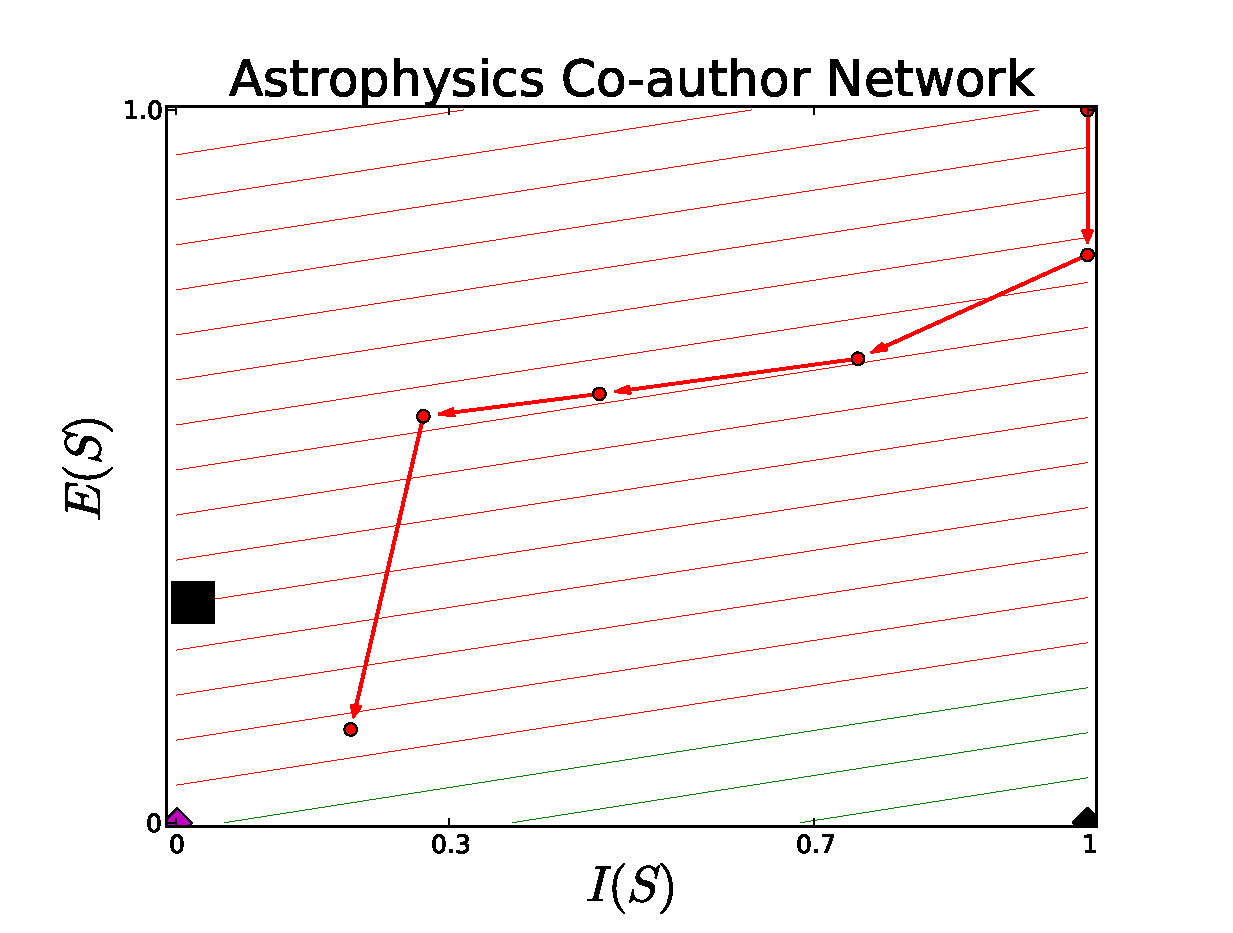
\includegraphics[width=1.5in]{Figures/linear_sets_astro}
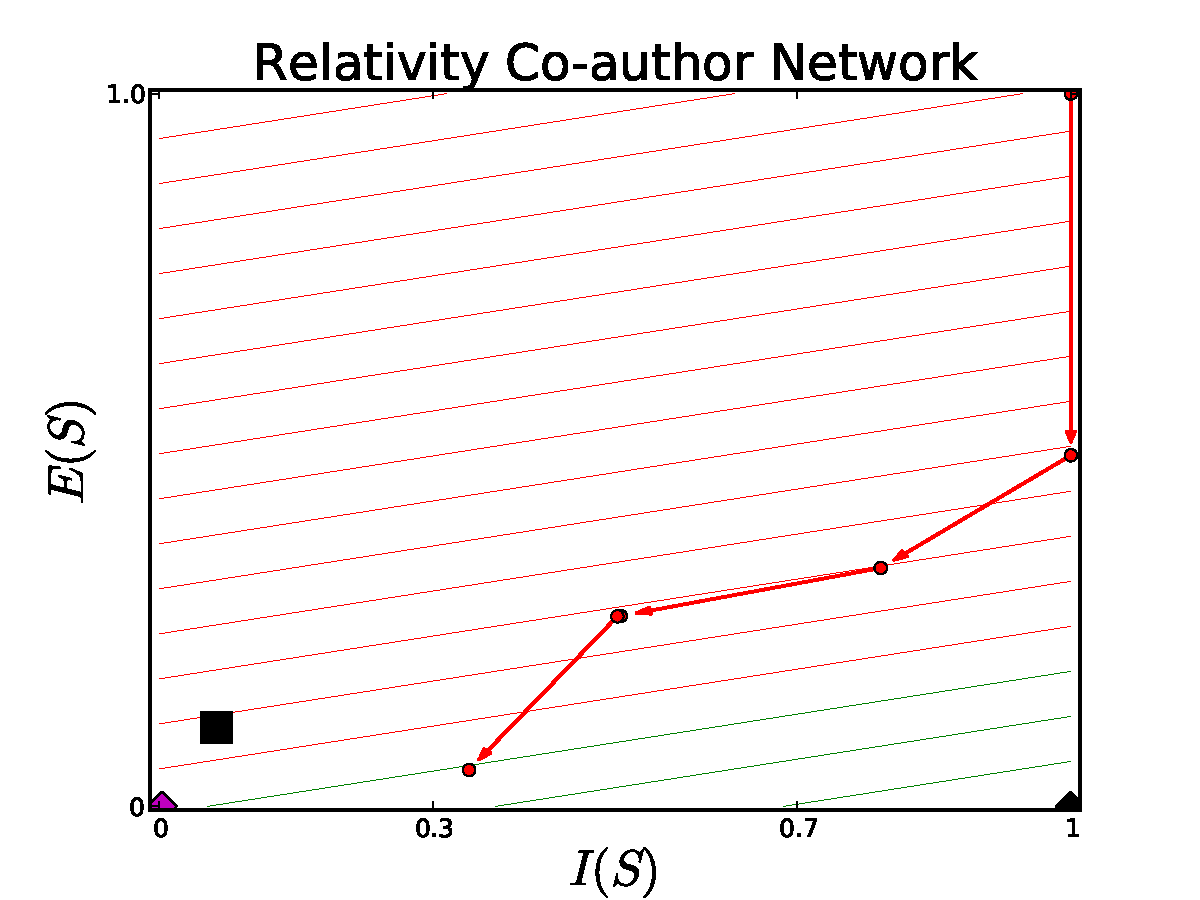
\includegraphics[width=1.5in]{Figures/linear_sets_relativity}
\caption{Black stars and squares are the sets of communities found by modularity}
\end{figure}
\end{frame}


\section{Parallel Technique for Large Complex Networks}



\begin{frame}\frametitle{Future}
\begin{block}{Small Network Paradigm}
\begin{center}
Is $C_1$ a good community within a set of communities $\{C_1, C_2, \dots\}$? \newline  \newline
{\it Does not parallelize.}
\end{center}
\end{block}
\begin{block}{Large Network Paradigm}
\begin{center}
Given a node $n$ and the set of nodes $X=\{n_1, n_2,\dots \}$, do they belong to the same community $C$? \newline \newline
{\it Easily parallelized.}
\end{center}
\end{block}
Large Network Paradigm has been used by [Mishra et al] and [Wang \& Hopcroft]
\end{frame}

\begin{frame}\frametitle{Characteristics}

\begin{definition}[$\chi_e$]
The number of edges a node has to members of a set of nodes, $X$, is characteristic $\chi_e$.
\begin{equation}
\chi_e(n, X) = |\mbox{Neighbors}(n)\cap X| \nonumber
\end{equation}
\end{definition}


\begin{definition}[$\chi_p$]
The proportion of total edges a node has to members of a set of nodes is characteristic $\chi_p$.
\begin{equation}
\chi_p(n, X) = \frac{|\mbox{Neighbors}(n)\cap X|}{\mbox{degree}(n)} \nonumber
\end{equation}
\end{definition}

If $\chi_p(n, X)$ {\bf OR} $\chi_e(n, X)$ is high, then $n \cup X$ belong to a community.

\end{frame}

\begin{frame}
\begin{table}
\centering
\begin{tabular}{cc}
Open Community & Closed Community \\
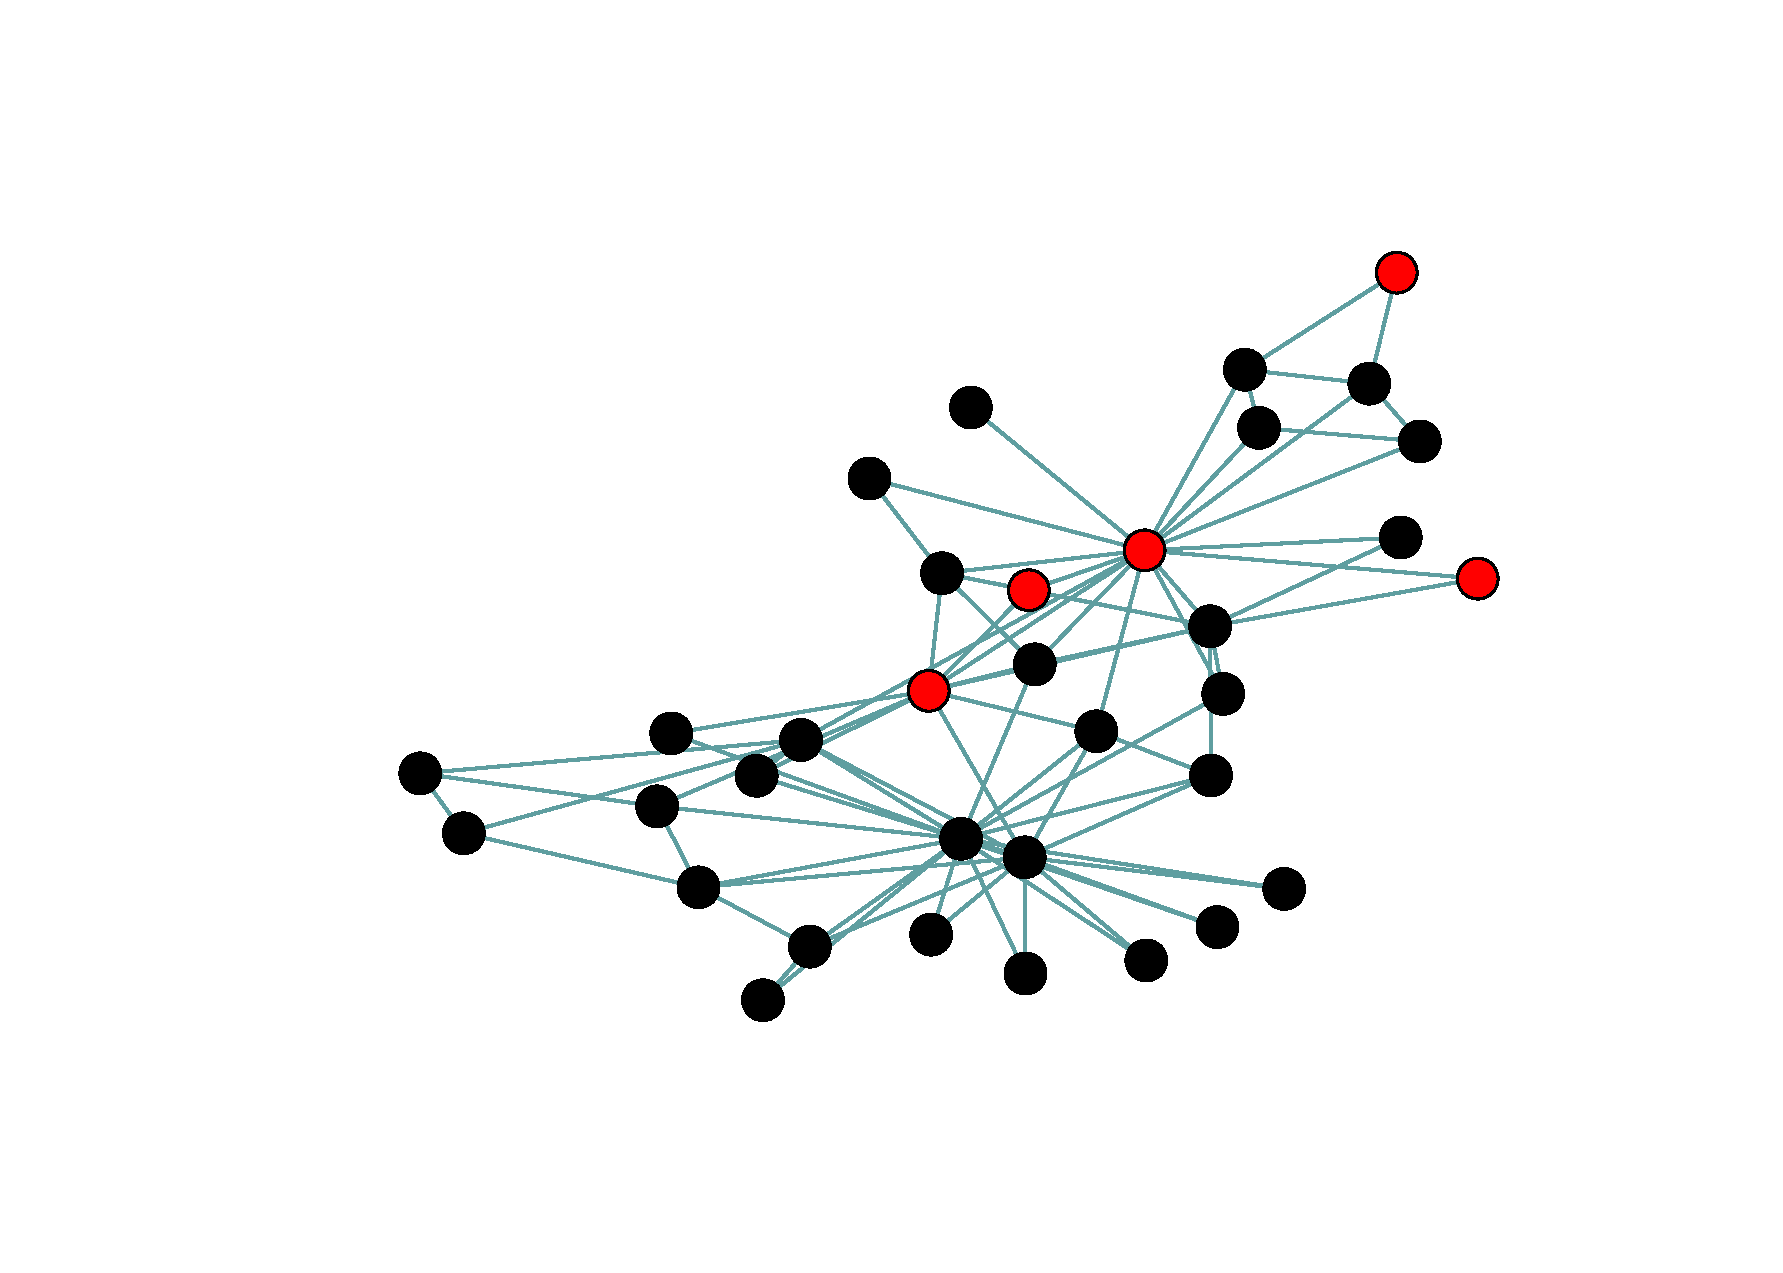
\includegraphics[width=1.4in]{Figures/open_community_drawn} &  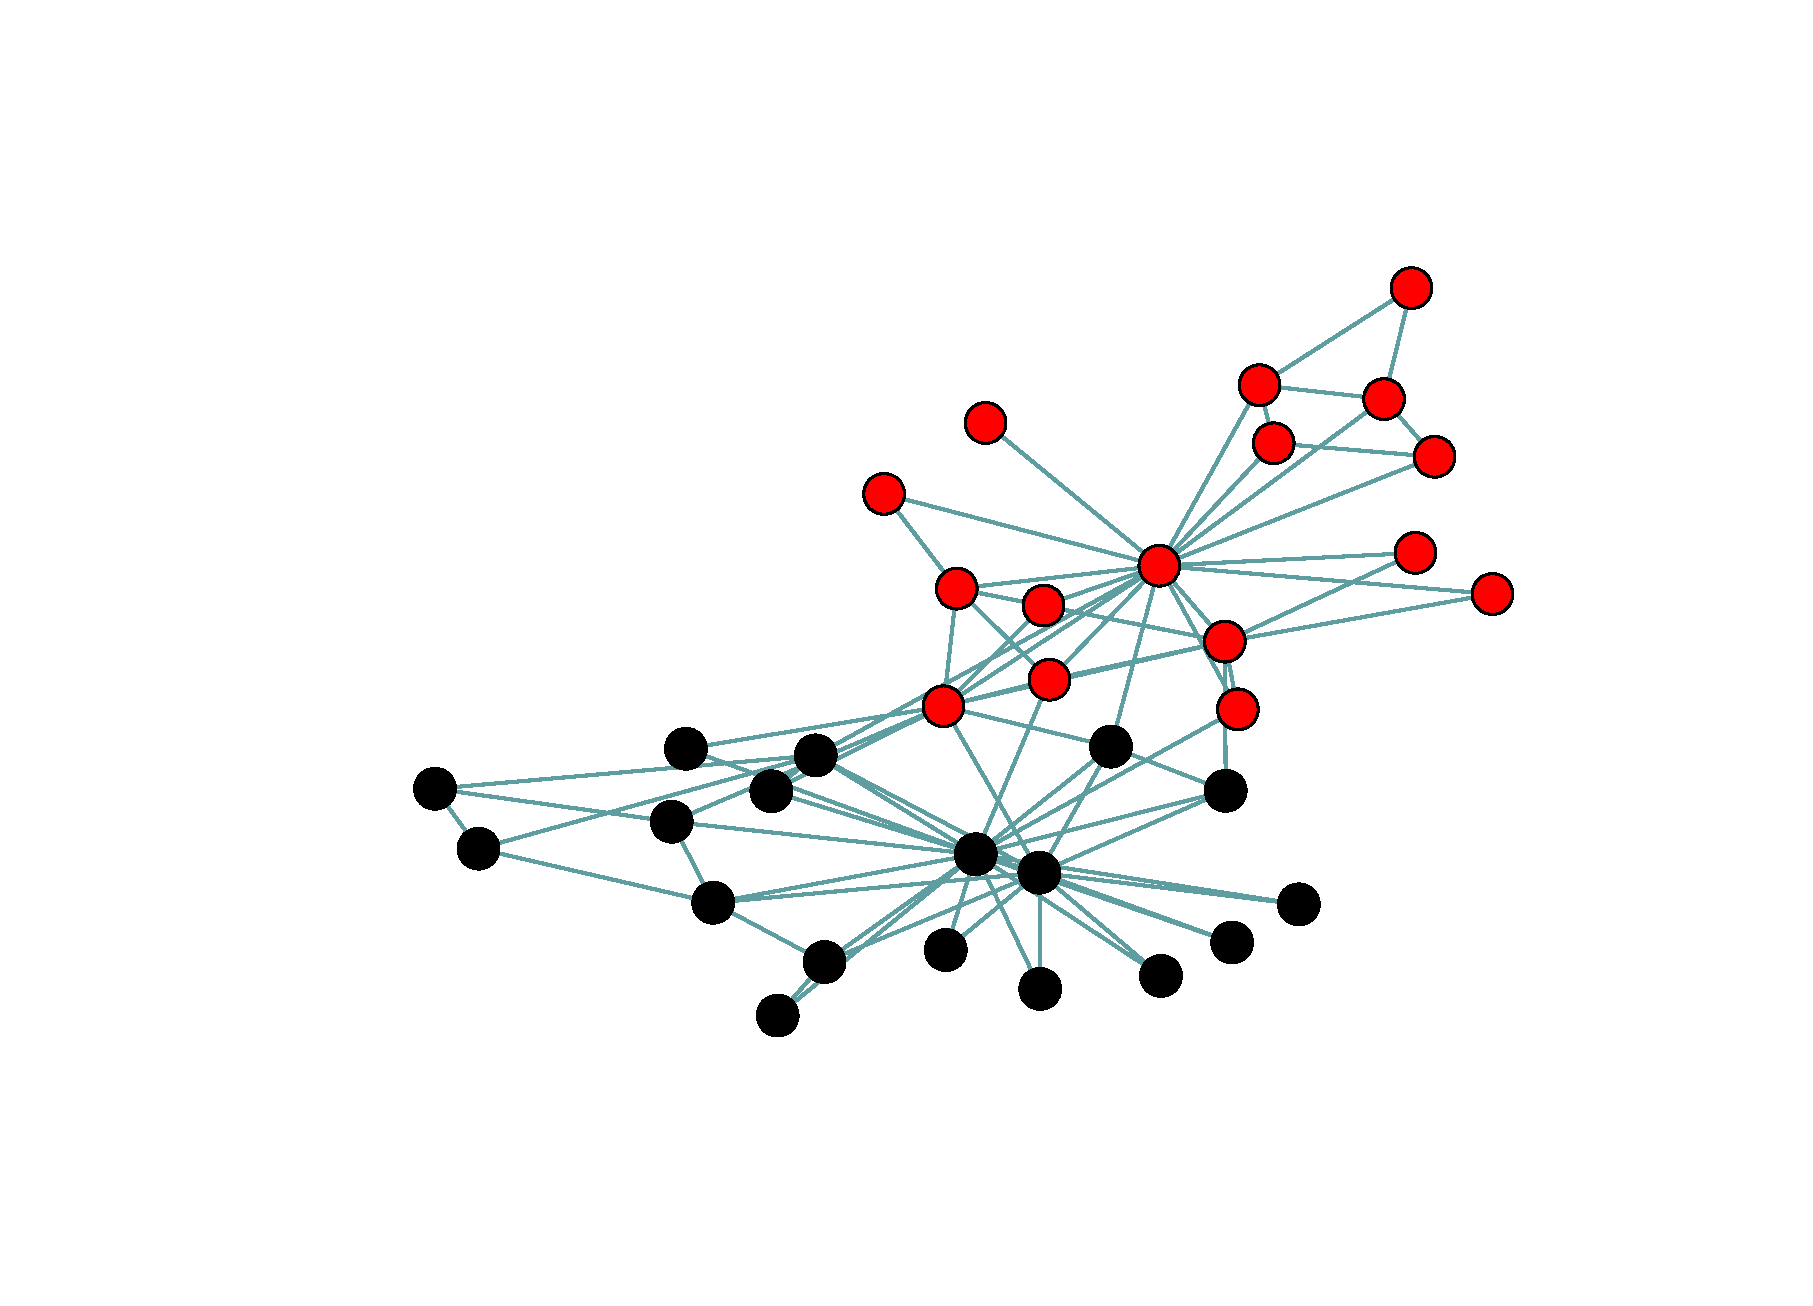
\includegraphics[width=1.4in]{Figures/closed_community_drawn} \\
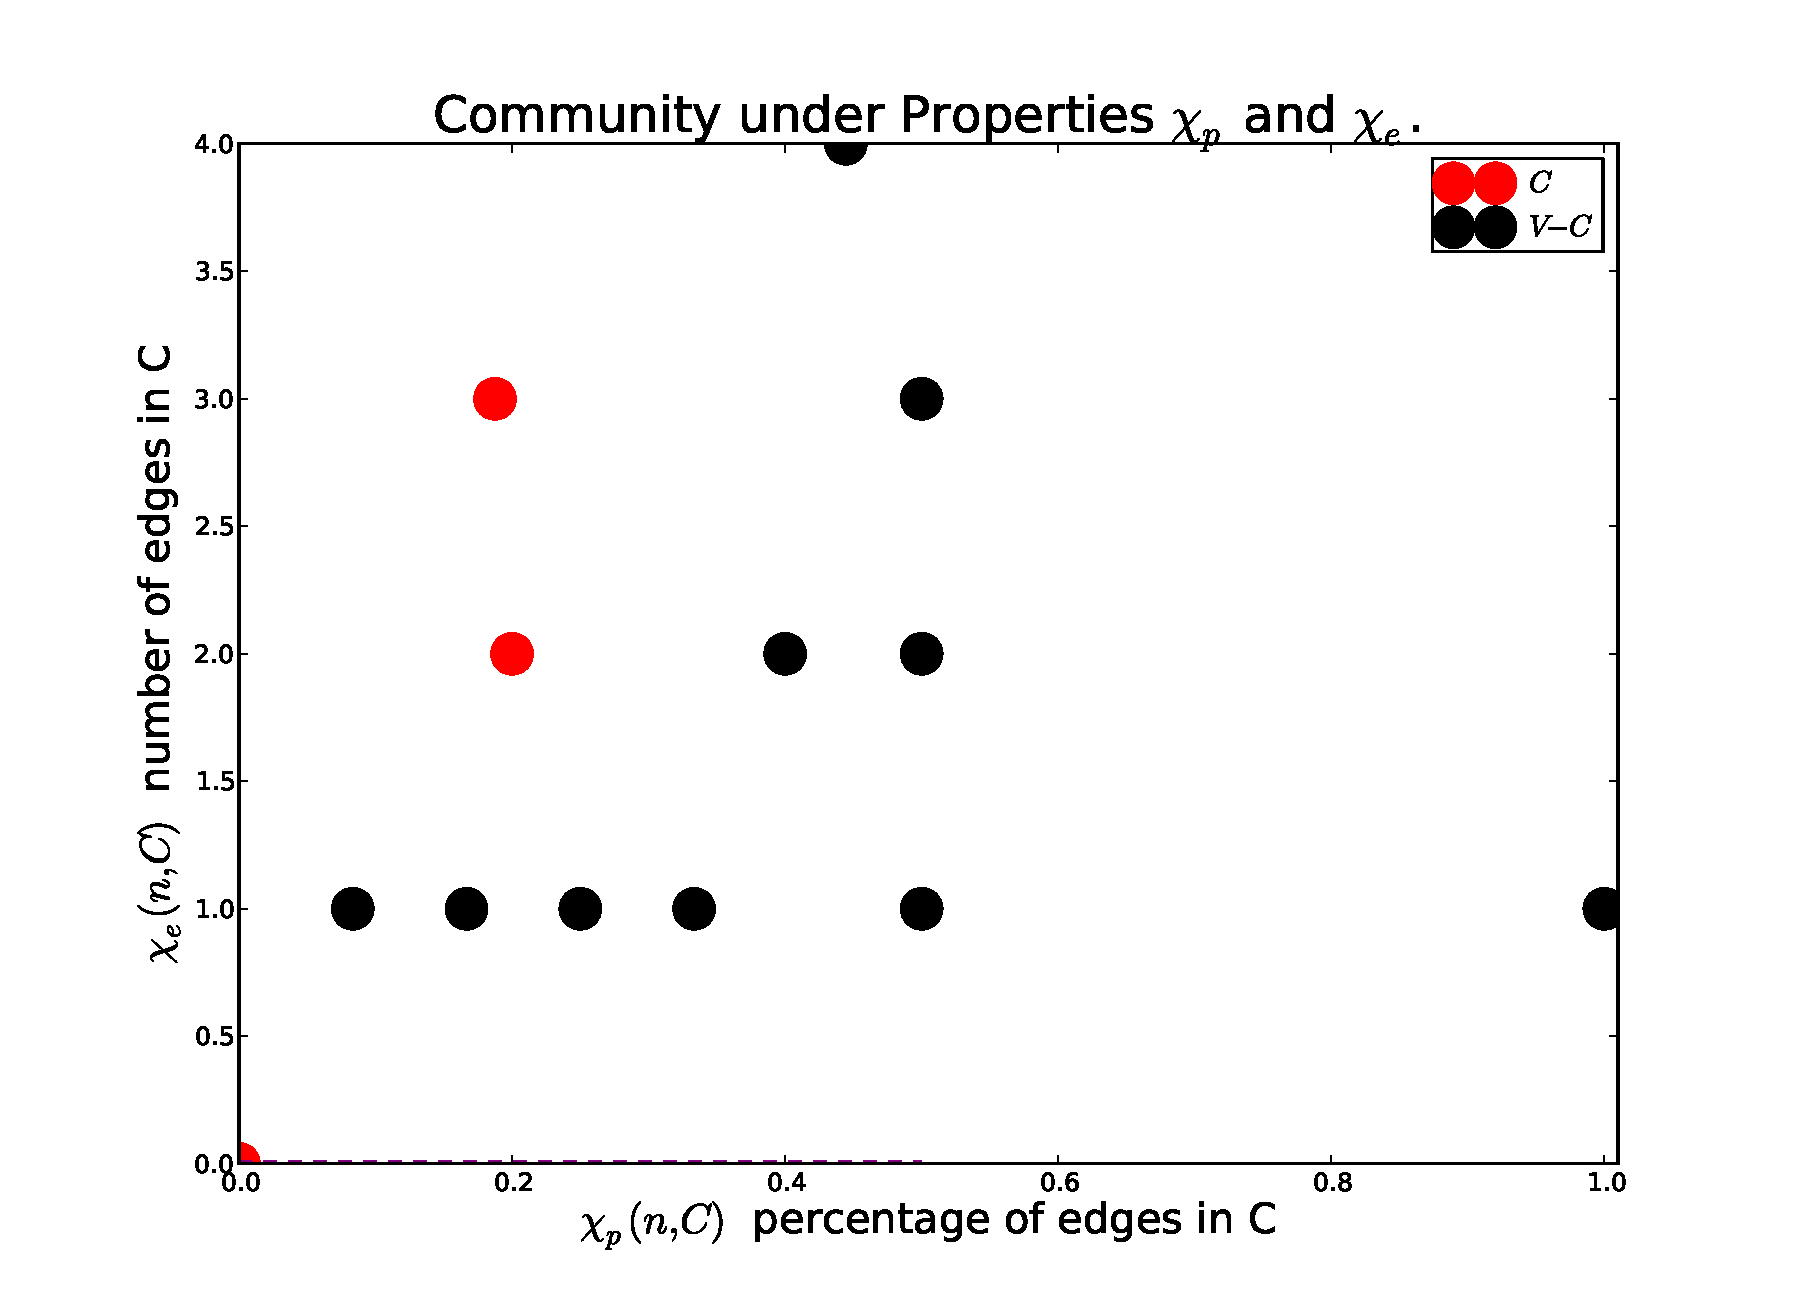
\includegraphics[width=2in]{Figures/open_community_e_p} &  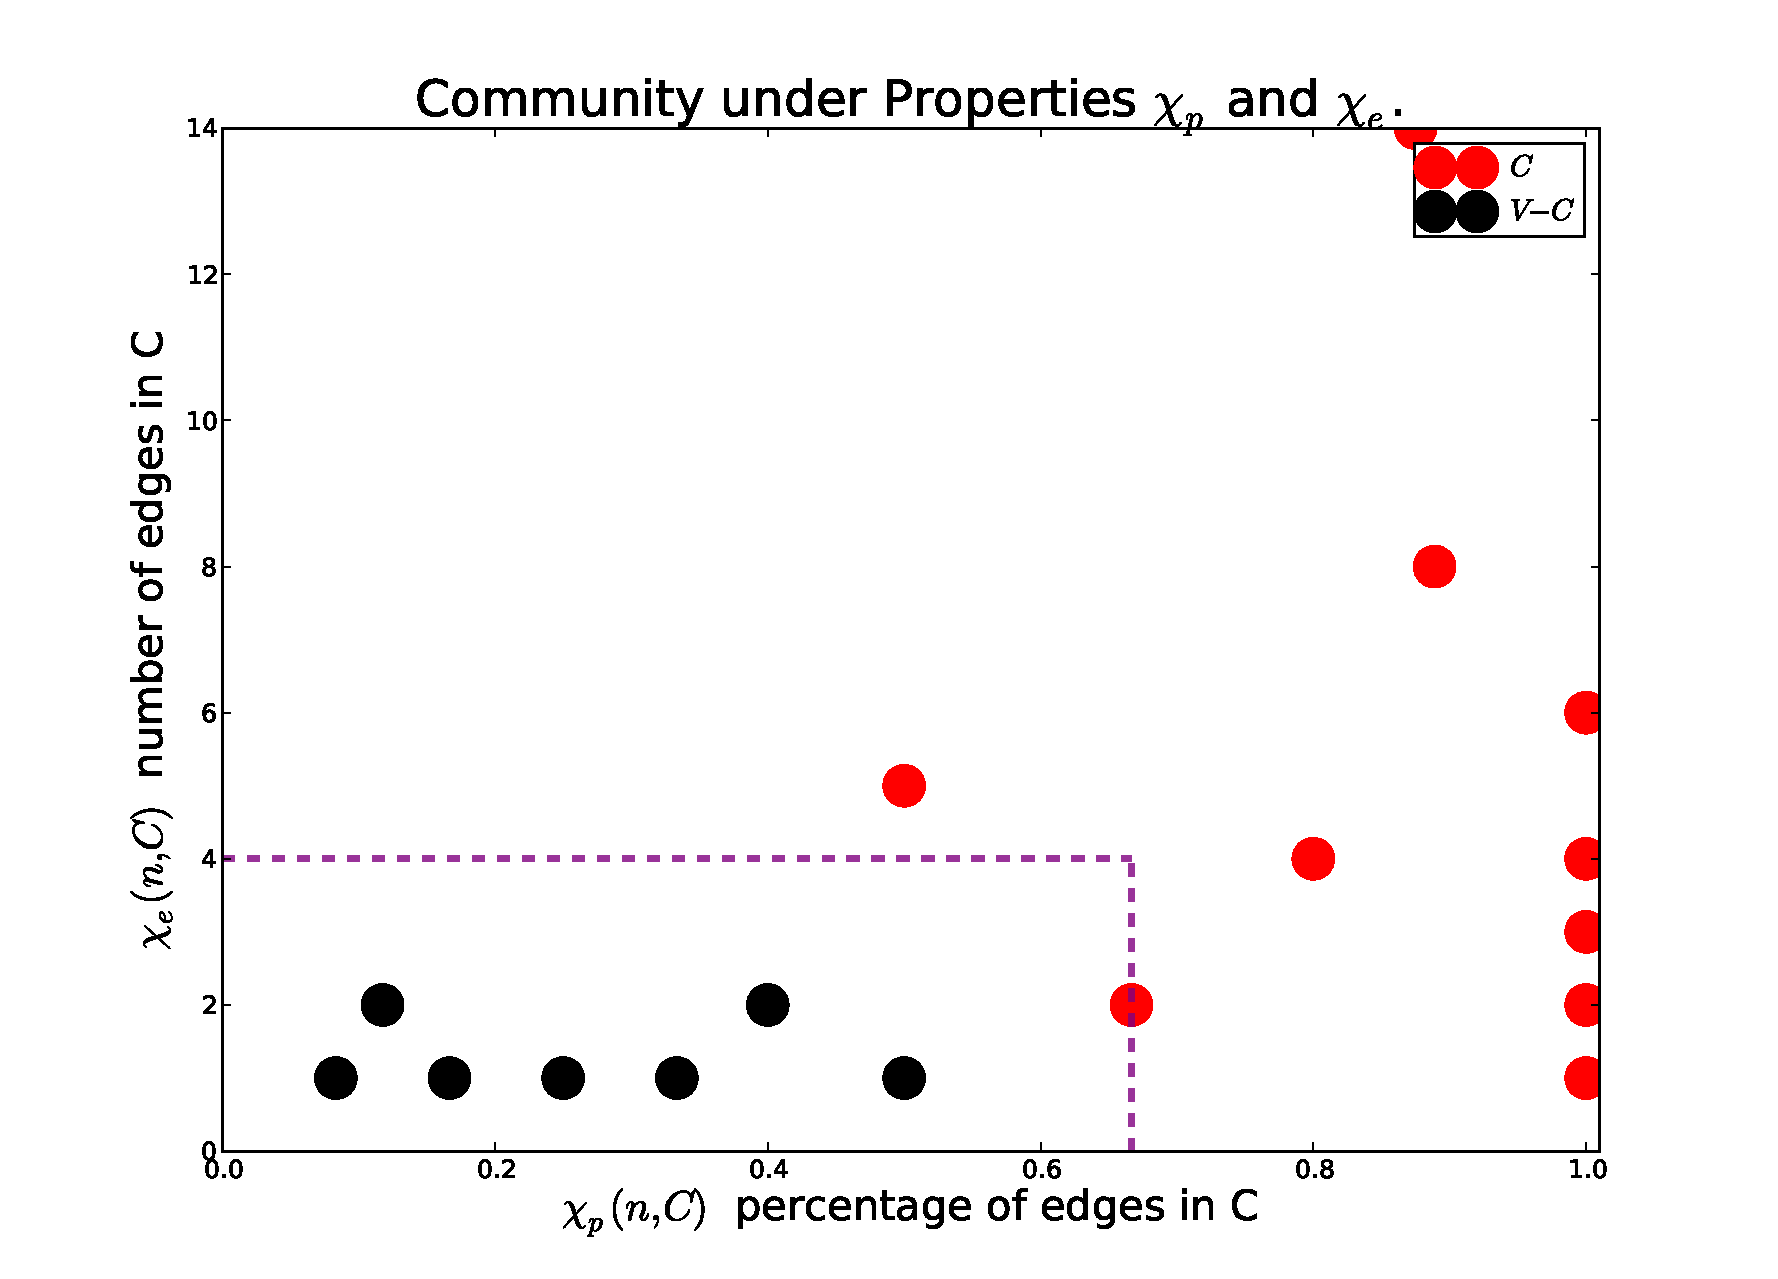
\includegraphics[width=2in]{Figures/closed_community_e_p} 
\end{tabular}
\end{table}
\end{frame}


\begin{frame}\frametitle{Seeds}

To begin need a set of nodes, $X$, that belong to the same community. \newline \newline

\begin{definition}[Seed]
A set of nodes that belong to the same community. \newline
\end{definition}
Strongest seeds are near cliques.  Easy to find. Can be done in parallel.
\end{frame}



\begin{frame}\frametitle{Expansion}

Given the set of seeds, we can expand them in parallel to find closed communities. \newline 

\begin{algorithmic}
	\STATE Communities$=[]$
	\FOR{$X \in $ Seeds}
		\WHILE{there exists $n \notin X$ with a high $\chi_e(n, X)$ {\bf OR} $\chi_p(n, X)$}
			\STATE $X \leftarrow X \cup \{n\}$
		\ENDWHILE
	\STATE Add $X$ to Communities
	\ENDFOR
\end{algorithmic}
To optimize select $n$ with the maximum $\chi_e(n, X)$ {\bf OR} $\chi_p(n, X)$.

Variations exist to find larger communities.  

\end{frame}


\begin{frame}\frametitle{Correctness of Expansion}
In the thesis we find closed form solutions for:
\begin{eqnarray*}
 P(n \cup X \subset C &|& n \mbox{ has max } \chi_e(n, X)) \\
 P(n \cup X \subset C &|& \chi_p(n, X))
\end{eqnarray*}
\newline

\begin{table}[t]
\centering
\begin{tabular}{ccc}
Select & Binomial Random Graph & Power Law Graph \\
node $n$ has $\max \{\chi_e\}$ & $> 94 \%$&  $> 90 \%$ \\
$\chi_p(n, X) = \frac{1}{2}$ & & 
\end{tabular}
\caption{Probability of Correctly Expanding a seed under unfavorable conditions.}
\end{table}

\end{frame}



\section{Applications}

\subsection{Physics Archive}

\begin{frame}\frametitle{Physics Archive}
We know the number of citations a paper makes is not related to the number of citations a paper receives[].
 Same is true for communities.
\begin{figure}
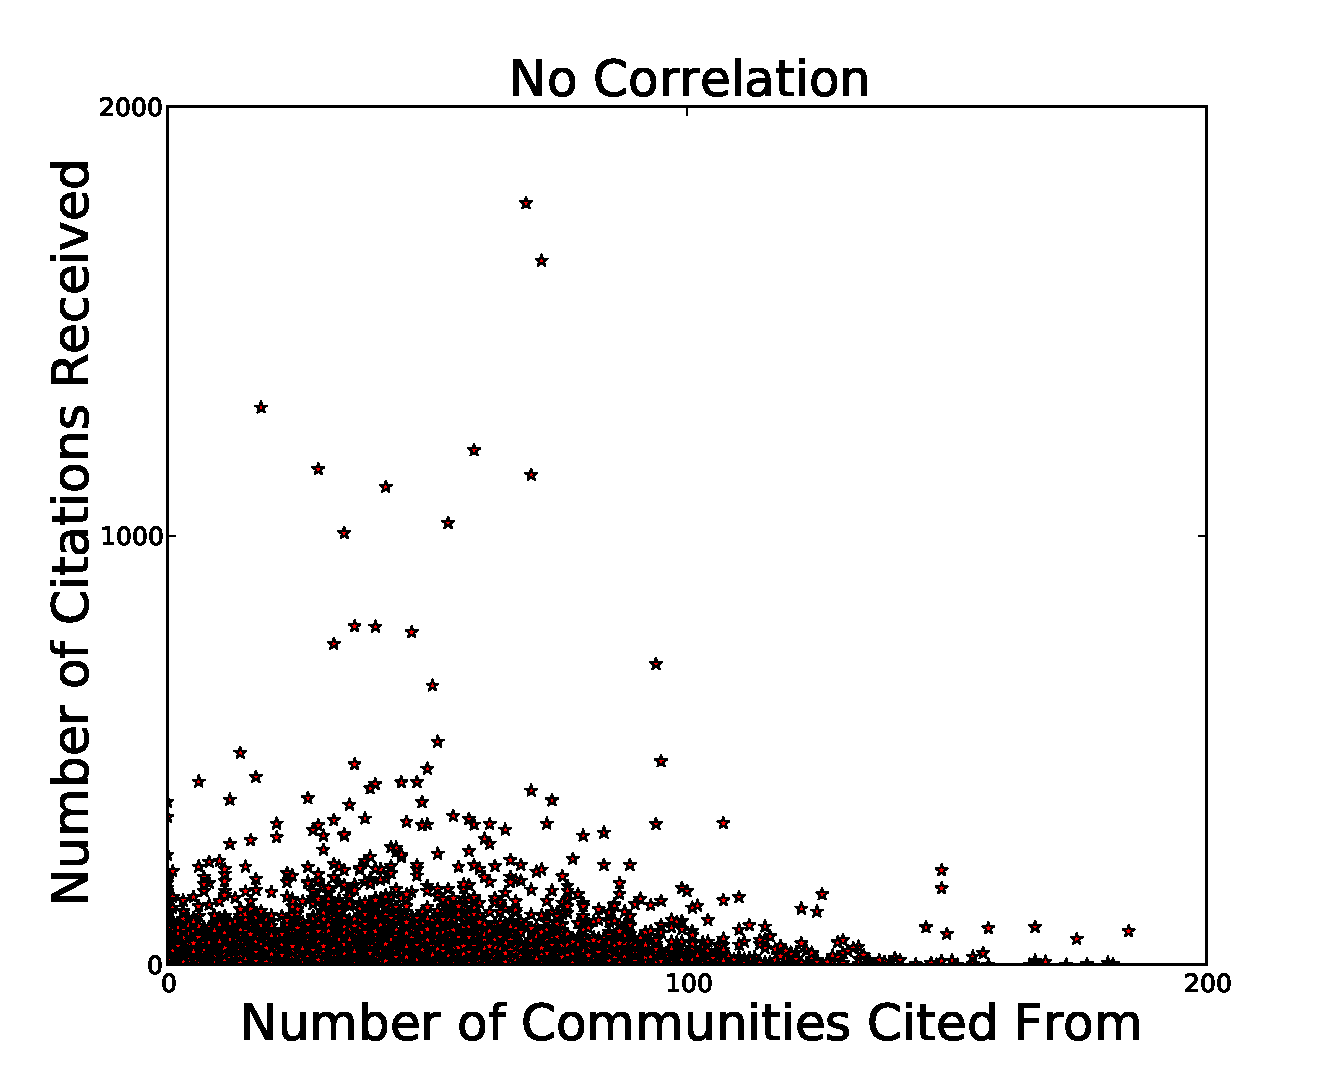
\includegraphics[width=2in]{Figures/communities_cites}
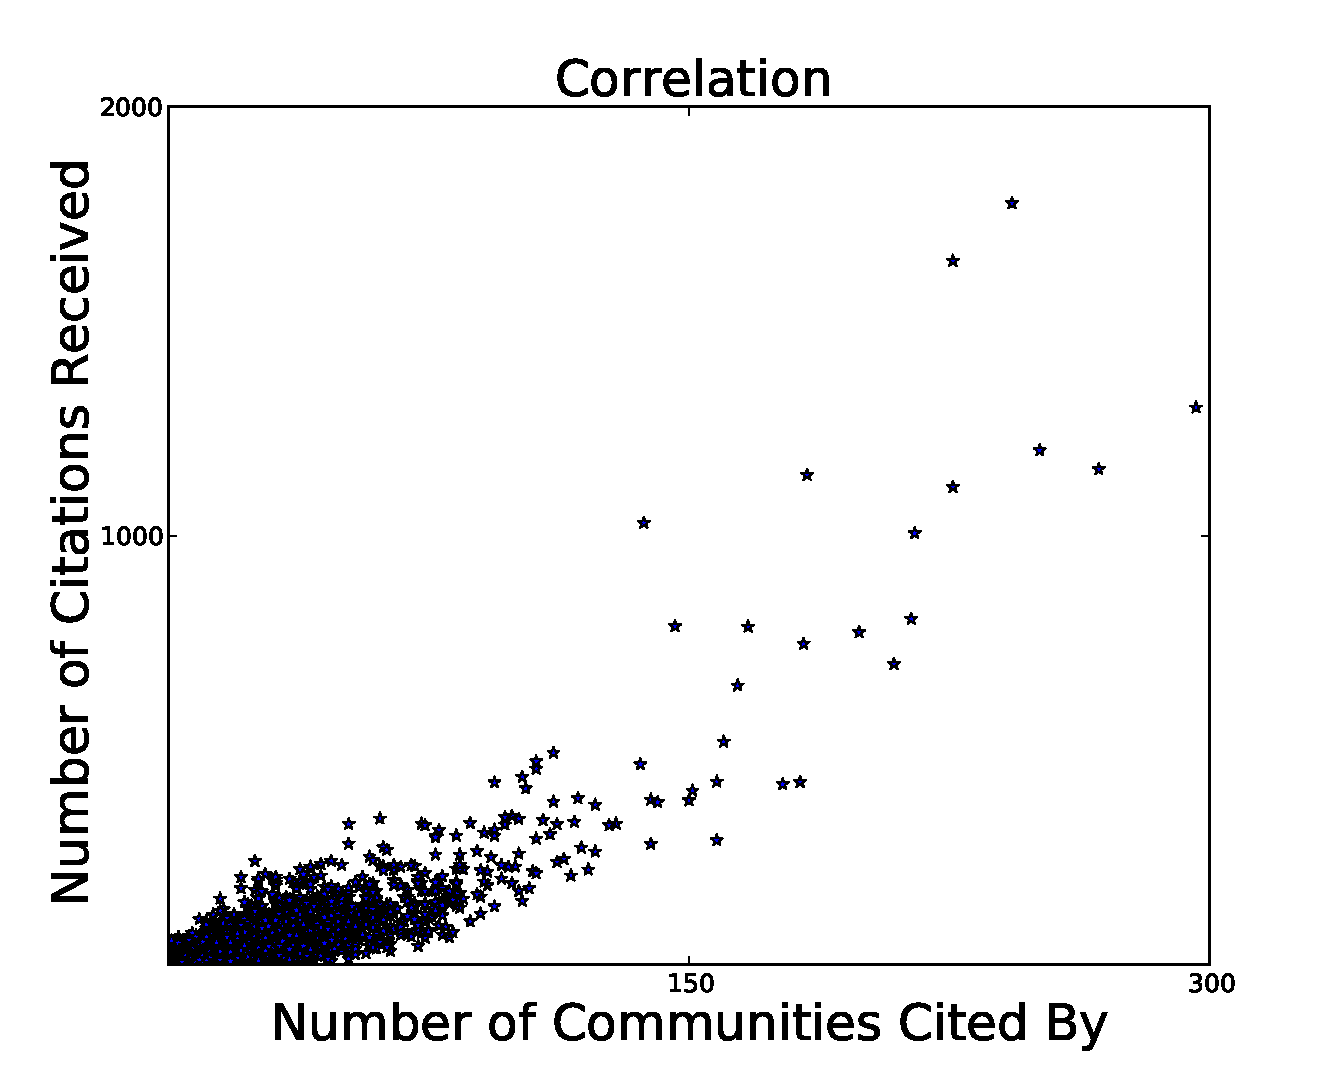
\includegraphics[width=2in]{Figures/communities_cited_by}
\end{figure}
But, the more communities a paper is cited by, is correlated with a paper's success.

Correlated with cross community journals - confirm.
\end{frame}


\begin{frame}\frametitle{Physics Archive}
JTODO include plot of communities evolving, we can now pick out the nodes corresponding to spanners, interpretors, etc
\end{frame}

\begin{frame}\frametitle{Physics Archive}
JTODO include diagram of number of communities a node belongs to follows a power law distribution
\end{frame}

\subsection{Wikipedia Voting}

\begin{frame}\frametitle{Wikipedia Voting, $2794$ elections}
\begin{figure}
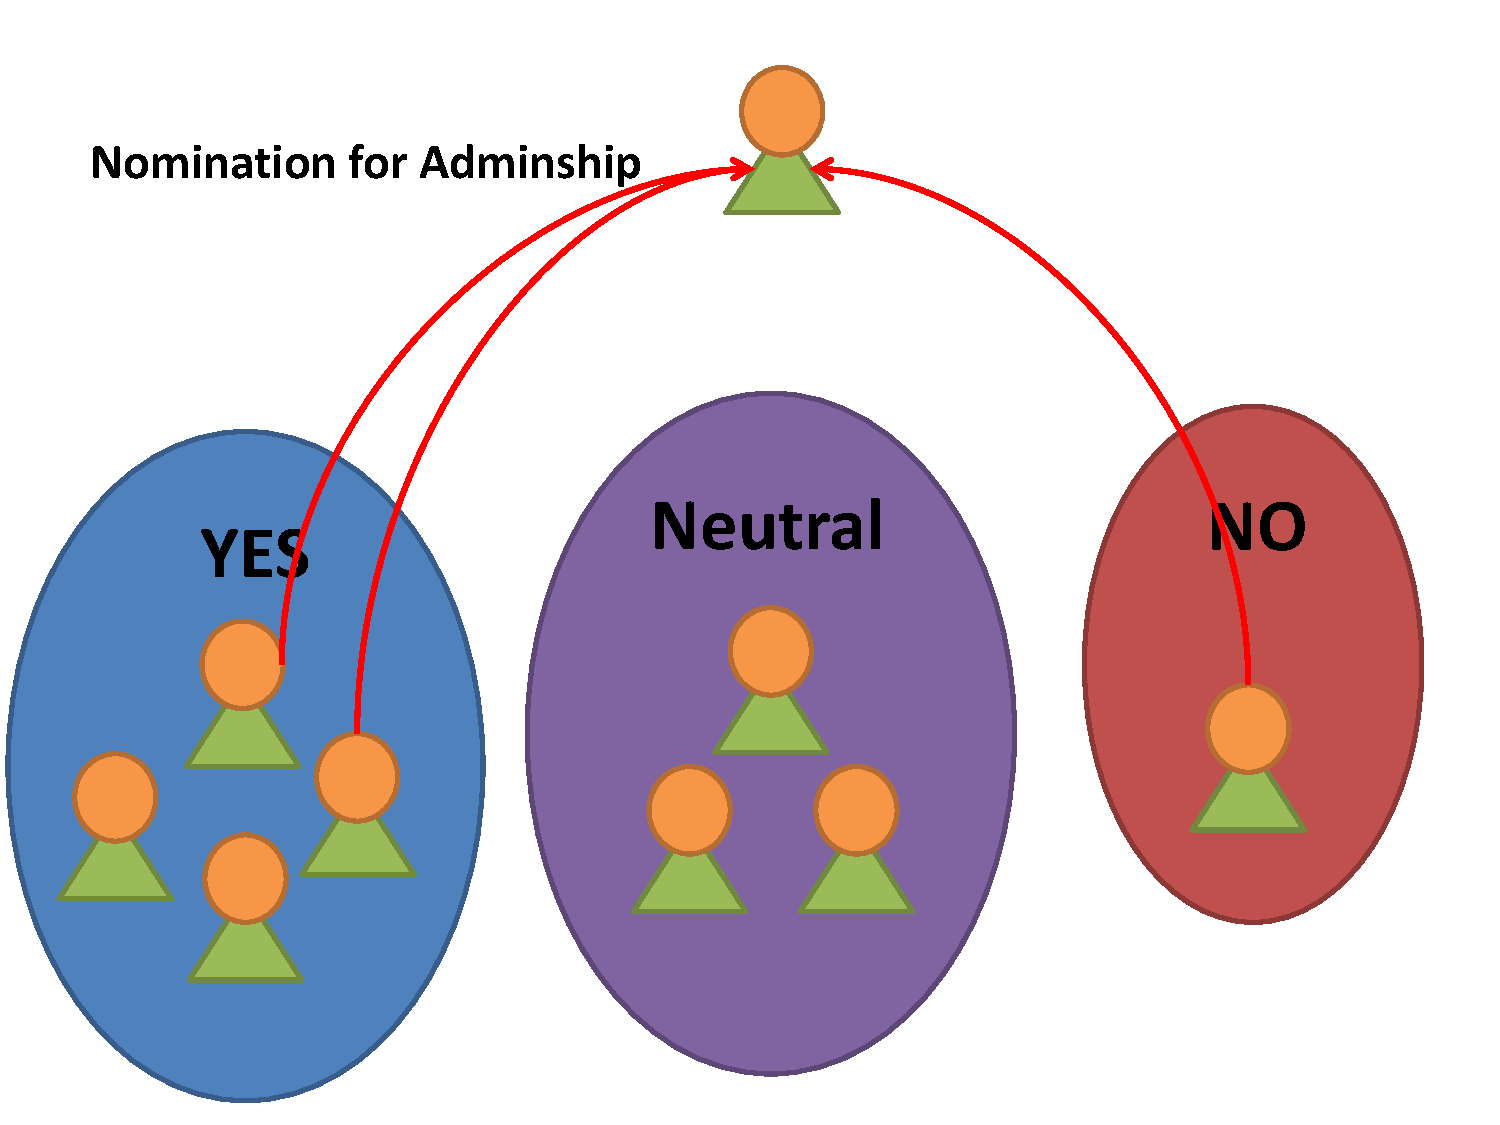
\includegraphics[width=2in]{Figures/wiki_votes}
\end{figure}
Network: $6287$ users that vote $114k$ times in $2794$ elections ({\it not everyone votes}).  There are $\approx 624$ communities, with an average size of $24$ users.

Communities are sets of user with similar voting patterns, in sign and frequency.  Users not in communities have erratic voting patterns.  The number of communities a user is in, follows a power law distribution.
\end{frame}


\begin{frame}\frametitle{Communities Predicting a User's Vote}

To predict how a user voted in an election:
\begin{itemize}
\item Remove the user's vote.
\item Calculate how the communities the user is in, voted.
\item Predict the user's vote with how a majority of the communities voted.
\end{itemize}


\begin{table}[t]
\centering
\begin{tabular}{cc}
Accuracy & Percentage of Votes Predicted \\ \hline
 $83\%$ & $60\%$ \\
$86\%$ & $13\%$\\
$95\%$ & $4\%$ 
\end{tabular}
\caption{The affect of smaller communities}
\end{table}

 [Leskovec, Huttenlocher, \& Kleinberg] attain $90 \%$ accuracy with a model for vote predictions.

\end{frame}

\begin{frame}\frametitle{Communities Predicting an Election's Outcome.}
We double the number of votes, by including votes with $90\%$ accuracy. \newline

\begin{block}{Election Prediction}
\begin{center}
If twice as many people voted, $7\%$ of elections would be overturned.
\end{center}
\end{block}

\begin{table}[t]
\centering
\begin{tabular}{ccc}
Did Vote & If More Users Voted & Type\\ \hline
$\{ \mbox{Yes: 158, No: 60}\}$ & $\{ \mbox{Yes: 498, No: 82}\}$ & False Negative \\
$\{ \mbox{Yes: 14, No: 6}\}$ & $\{ \mbox{Yes: 109, No: 25}\}$ & False Negative\\
$\{ \mbox{Yes: 45, No:7}\}$ & $\{ \mbox{Yes: 93, No: 38}\}$ & False Positive\\
\end{tabular}
\caption{Sample Changes in the Vote}
\end{table}
\begin{block}{Application}
\begin{center}
Use the communities to detect if a non-representative group is voting and alert Wikipedia Bureaucrats, who can overturn the election.
\end{center}
\end{block}

\end{frame}

\end{document}






% sample code to work with



\section{Section no.1} 
\begin{frame}\frametitle{Title} 
Each frame should have a title.
\end{frame}
\subsection{Subsection no.1.1  }
\begin{frame} 
Without title somethink is missing. 
\end{frame}


\section{Section no. 2} 
\subsection{Lists I}
\begin{frame}\frametitle{unnumbered lists}
\begin{itemize}
\item Introduction to  \LaTeX  
\item Course 2 
\item Termpapers and presentations with \LaTeX 
\item Beamer class
\end{itemize} 
\end{frame}

\begin{frame}\frametitle{lists with pause}
\begin{itemize}
\item Introduction to  \LaTeX \pause 
\item Course 2 \pause 
\item Termpapers and presentations with \LaTeX \pause 
\item Beamer class
\end{itemize} 
\end{frame}

\subsection{Lists II}
\begin{frame}\frametitle{numbered lists}
\begin{enumerate}
\item Introduction to  \LaTeX  
\item Course 2 
\item Termpapers and presentations with \LaTeX 
\item Beamer class
\end{enumerate}
\end{frame}

\begin{frame}\frametitle{numbered lists with pause}
\begin{enumerate}
\item Introduction to  \LaTeX \pause 
\item Course 2 \pause 
\item Termpapers and presentations with \LaTeX \pause 
\item Beamer class
\end{enumerate}
\end{frame}

\section{Section no.3} 
\subsection{Tables}
\begin{frame}\frametitle{Tables}
\begin{tabular}{|c|c|c|}
\hline
\textbf{Date} & \textbf{Instructor} & \textbf{Title} \\
\hline
WS 04/05 & Sascha Frank & First steps with  \LaTeX  \\
\hline
SS 05 & Sascha Frank & \LaTeX \ Course serial \\
\hline
\end{tabular}
\end{frame}


\begin{frame}\frametitle{Tables with pause}
\begin{tabular}{c c c}
A & B & C \\ 
\pause 
1 & 2 & 3 \\  
\pause 
A & B & C \\ 
\end{tabular} 
\end{frame}


\section{Section no. 4}
\subsection{blocs}
\begin{frame}\frametitle{blocs}

\begin{block}{title of the bloc}
bloc text
\end{block}

\begin{exampleblock}{title of the bloc}
bloc text
\end{exampleblock}


\begin{alertblock}{title of the bloc}
bloc text
\end{alertblock}
\end{frame}

\section{Section no. 5}
\subsection{split screen}

\begin{frame}\frametitle{splitting screen}
\begin{columns}
\begin{column}{5cm}
\begin{itemize}
\item Beamer 
\item Beamer Class 
\item Beamer Class Latex 
\end{itemize}
\end{column}
\begin{column}{5cm}
\begin{tabular}{|c|c|}
\hline
\textbf{Instructor} & \textbf{Title} \\
\hline
Sascha Frank &  \LaTeX \ Course 1 \\
\hline
Sascha Frank &  Course serial  \\
\hline
\end{tabular}
\end{column}
\end{columns}
\end{frame}

\subsection{Pictures} 
\begin{frame}\frametitle{pictures in latex beamer class}
\begin{figure}
\includegraphics[scale=0.5]{PIC1} 
\caption{show an example picture}
\end{figure}
\end{frame}

\subsection{joining picture and lists} 

\begin{frame}
\frametitle{pictures and lists in beamer class}
\begin{columns}
\begin{column}{5cm}
\begin{itemize}
\item<1-> subject 1
\item<3-> subject 2
\item<5-> subject 3
\end{itemize}
\vspace{3cm} 
\end{column}
\begin{column}{5cm}
\begin{overprint}
\includegraphics<2>{PIC1}
\includegraphics<4>{PIC2}
\includegraphics<6>{PIC3}
\end{overprint}
\end{column}
\end{columns}
\end{frame}


\subsection{pictures which need more space} 
\begin{frame}[plain]
\frametitle{plain, or a way to get more space}
\begin{figure}
\includegraphics[scale=0.5]{PIC1} 
\caption{show an example picture}
\end{figure}
\end{frame}
